\documentclass[a4paper, 10pt, ]{article}

\usepackage[slovak]{babel}





\usepackage[utf8]{inputenc}
\usepackage[T1]{fontenc}

\usepackage[left=4cm,
			right=4cm,
            % left=2.5cm,
			% right=5.5cm,
			top=2.1cm,
			bottom=2.6cm,
			footskip=7.5mm,
			% twoside,
			marginparwidth=3.0cm,
			%showframe,
			]{geometry}

\usepackage{graphicx}
\usepackage[dvipsnames]{xcolor}
% https://en.wikibooks.org/wiki/LaTeX/Colors


% ------------------------------

\usepackage{lmodern}

\usepackage[tt={oldstyle=false,proportional=true,monowidth}]{cfr-lm}

% ------------------------------

\usepackage{amsmath}
\usepackage{amssymb}
\usepackage{amsthm}

\usepackage{booktabs}
\usepackage{multirow}
\usepackage{array}
\usepackage{dcolumn}


\usepackage[singlelinecheck=true]{subfig}


% ------------------------------


\def\naT{\mathsf{T}}

\hyphenpenalty=6000
\tolerance=1000




% ------------------------------


\makeatletter

	\def\@seccntformat#1{\protect\makebox[0pt][r]{\csname the#1\endcsname\hspace{4mm}}}

	\def\cleardoublepage{\clearpage\if@twoside \ifodd\c@page\else
	\hbox{}
	\vspace*{\fill}
	\begin{center}
	\phantom{}
	\end{center}
	\vspace{\fill}
	\thispagestyle{empty}
	\newpage
	\if@twocolumn\hbox{}\newpage\fi\fi\fi}

	\newcommand\figcaption{\def\@captype{figure}\caption}
	\newcommand\tabcaption{\def\@captype{table}\caption}

\makeatother


% ------------------------------




\usepackage{fancyhdr}
\fancypagestyle{plain}{%
\fancyhf{} % clear all header and footer fields
\fancyfoot[C]{\sffamily {\bfseries \thepage}\ | {\scriptsize\oznacenieCasti}}
\renewcommand{\headrulewidth}{0pt}
\renewcommand{\footrulewidth}{0pt}}
\pagestyle{plain}


% ------------------------------


\usepackage{titlesec}
\titleformat{\paragraph}[hang]{\sffamily  \bfseries}{}{0pt}{}
\titlespacing*{\paragraph}{0mm}{3mm}{1mm}
\titlespacing*{\subparagraph}{0mm}{3mm}{1mm}

\titleformat*{\section}{\sffamily\Large\bfseries}
\titleformat*{\subsection}{\sffamily\large\bfseries}
\titleformat*{\subsubsection}{\sffamily\normalsize\bfseries}






% ------------------------------

\PassOptionsToPackage{hyphens}{url}
\usepackage[pdfauthor={},
			pdftitle={},
			pdfsubject={},
			pdfkeywords={},
			% hidelinks,
			colorlinks=false,
			breaklinks,
			]{hyperref}


% ------------------------------


\graphicspath{%
{../fig_standalone/}%
{../../PY/fig/}%
{../../PY/jupynotex/fig/}%
{../../ML/fig/}%
{./fig/}%
}



% ------------------------------

\usepackage{enumitem}

\usepackage{lettrine}

% ------------------------------


\usepackage{microtype}


% ------------------------------

\usepackage[titles]{tocloft}

\setlength{\cftsecindent}{-12mm}
\setlength{\cftsecnumwidth}{12mm}
\renewcommand{\cftsecpresnum}{\hfill}
\renewcommand{\cftsecaftersnum}{\hspace{4mm}}

\setlength{\cftsubsecindent}{-12mm}
\setlength{\cftsubsecnumwidth}{16mm} % 12 + 4
\renewcommand{\cftsubsecpresnum}{\hfill}
\renewcommand{\cftsubsecaftersnum}{\hspace{8mm}} % 4 + 4 mm

\setlength{\cftsubsubsecindent}{-12mm}
\setlength{\cftsubsubsecnumwidth}{20mm} % 12 + 4 + 4
\renewcommand{\cftsubsubsecpresnum}{\hfill}
\renewcommand{\cftsubsubsecaftersnum}{\hspace{12mm}} % 4 + 4 + 4 mm

\renewcommand{\cftsecpagefont}{\lstyle \bfseries}
\renewcommand{\cftsubsecpagefont}{\lstyle}
\renewcommand{\cftsubsubsecpagefont}{\lstyle}



\setlength{\cftparaindent}{-16mm}
\setlength{\cftparanumwidth}{28mm} % 16 + 4 + 4 + 4
\renewcommand{\cftparapresnum}{\hfill}
\renewcommand{\cftparaaftersnum}{\hspace{16mm}} % 4 + 4 + 4 + 4 mm








% ------------------------------

\usepackage{listings}



\renewcommand{\lstlistingname}{Výpis kódu}
\renewcommand{\lstlistlistingname}{Výpisy kódu}




%New colors defined below
\definecolor{codegreen}{rgb}{0,0.6,0}
\definecolor{codegray}{rgb}{0.5,0.5,0.5}
\definecolor{codepurple}{rgb}{0.58,0,0.82}
\definecolor{backcolour}{rgb}{0.95,0.95,0.95}

%Code listing style named "mystyle"
\lstdefinestyle{mystyle}{
  backgroundcolor=\color{backcolour},
  commentstyle=\fontfamily{lmtt}\fontsize{8.5pt}{8.75pt}\selectfont\color{codegreen},
  keywordstyle=\fontfamily{lmtt}\fontsize{8.5pt}{8.75pt}\selectfont\bfseries\color{Blue},
  stringstyle=\fontfamily{lmtt}\fontsize{8.5pt}{8.75pt}\selectfont\color{codepurple},
  basicstyle=\fontfamily{lmtt}\fontsize{8.5pt}{8.75pt}\selectfont,
  breakatwhitespace=false,
  breaklines=true,
  captionpos=t,
  keepspaces=true,
  numbers=left,
  numbersep=4mm,
  numberstyle=\fontfamily{lmtt}\fontsize{8.5pt}{8.75pt}\selectfont\color{lightgray},
  showspaces=false,
  showstringspaces=false,
  showtabs=false,
  tabsize=2,
  % xleftmargin=10pt,
  framesep=10pt,
  language=Python,
  escapechar=|,
}


\lstset{
    inputencoding=utf8,
    extendedchars=true,
    literate=%
    {á}{{\'a}}1
    {č}{{\v{c}}}1
    {ď}{{\v{d}}}1
    {é}{{\'e}}1
    {ě}{{\v{e}}}1
    {í}{{\'i}}1
    {ň}{{\v{n}}}1
    {ó}{{\'o}}1
    {ř}{{\v{r}}}1
    {š}{{\v{s}}}1
    {ť}{{\v{t}}}1
    {ú}{{\'u}}1
    {ů}{{\r{u}}}1
    {ý}{{\'y}}1
    {ž}{{\v{z}}}1
    {Á}{{\'A}}1
    {Č}{{\v{C}}}1
    {Ď}{{\v{D}}}1
    {É}{{\'E}}1
    {Ě}{{\v{E}}}1
    {Í}{{\'I}}1
    {Ň}{{\v{N}}}1
    {Ó}{{\'O}}1
    {Ř}{{\v{R}}}1
    {Š}{{\v{S}}}1
    {Ť}{{\v{T}}}1
    {Ú}{{\'U}}1
    {Ů}{{\r{U}}}1
    {Ý}{{\'Y}}1
    {Ž}{{\v{Z}}}1
    {ô}{{\^{o}}}1
}


% ------------------------------


\usepackage{caption}

\DeclareCaptionFormat{odsadene}{\protect\makebox[0pt][r]{#1#2\hspace{4mm}}#3\par}
\DeclareCaptionLabelSeparator{lendvojbodka}{:}
% \DeclareCaptionFont{lightgray}{\color{lightgray}}
\DeclareCaptionFont{lightgray}{\fontfamily{lmtt}\fontsize{8.5pt}{8.75pt}\selectfont\color{lightgray}}

\captionsetup[lstlisting]{format=odsadene, labelsep=lendvojbodka, justification=raggedright, singlelinecheck=false, labelfont={sf, lightgray},}


% ------------------------------





% ------------------------------

\usepackage[backend=biber,
            style=numeric,
            sorting=none,
            ]{biblatex}
\DeclareSourcemap{
    \maps[datatype=bibtex]{
        \map{
        \step[fieldset=note, null]
        }
        \map{
        \step[fieldset=file, null]
        }        
        % \map{
        % \step[fieldset=url, null]        
        % }
        \map{
        \step[fieldset=eprint, null]
        }
    }
}


\addbibresource{E:/_CurrentContent/01_work_repo/bibLaTeXDB/bibLaTeXDB.bib} % nonpublic data





\def\oznacenieCasti{MRS10 - ZS2025}


\usepackage{longtable}




\begin{document}


\lstset{%
style=mystyle,
rangebeginprefix=\#\#\#\ cellB\ ,%
rangebeginsuffix=\ \#\#\#,%
rangeendprefix=\#\#\#\ cellE\ ,%
rangeendsuffix=\ \#\#\#,%
includerangemarker=false,
}





\fontsize{12pt}{22pt}\selectfont

\centerline{\textsf{Modelovanie a riadenie systémov} \hfill \textsf{\oznacenieCasti}}

\fontsize{18pt}{22pt}\selectfont





\begin{flushleft}
	\textbf{\textsf{Uzavretý regulačný obvod\\a~PID regulátor}}
\end{flushleft}





\normalsize

\bigskip

{\hypersetup{hidelinks}

\tableofcontents

}

\bigskip

\vspace{18pt}



\noindent
\lettrine[lines=1, nindent=1pt, loversize=0.0]{C}{ieľom} 
textu je sprostredkovanie úvodných informácií ku konceptu \emph{uzavretého regulačného obvodu} (URO). Skladá sa z riadeného systému a riadiaceho systému. Ak sme sa v predchádzajúcich textoch venovali primárne matematickému modelovaniu systémov, týkalo sa to predovšetkým riadeného systému v URO. Príkladom riadiaceho systému v URO je v tomto texte \emph{PID regulátor}.

\section{O regulačnom obvode}

Regulačný obvod sa vo všeobecnosti skladá z riadiaceho systému a z riadeného systému. Zahŕňa tri základné signály. Výstupnú veličinu $y(t)$, akčný zásah $u(t)$ a referenčný signál $r(t)$. Schematicky sa znázorňuje nasledovne:

\begin{center}

    \vbox{%
    \makebox[\textwidth][c]{%
	% 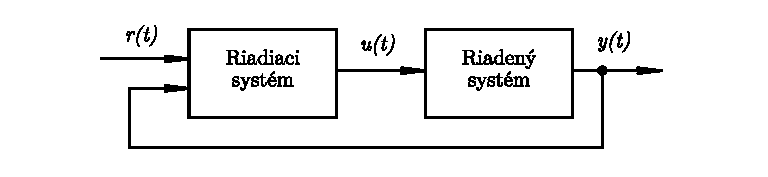
\includegraphics{schURO_vseob.pdf}
    \input{../fig_standalone/schURO_vseob.pdf_tex}
	}

	\figcaption{Všeobecný uzavretý regulačný obvod.}
    \label{schURO_vseob.pdf}
    }
	
\end{center}

Výstupom riadeného systému je veličina, ktorá, okrem iného, hovorí o splnení cieľa riadenia. Cieľom riadenia napríklad je, aby táto veličina dosiahla istú hodnotu, prípadne aby priebeh tejto veličiny v~čase vykazoval isté dynamické vlastnosti, a~podobne. Pre skrátenie sa práve táto veličina nazýva ako výstupná veličina (celého obvodu). Označuje sa $y(t)$.

Úlohou riadiaceho systému je splniť cieľ riadenia. Výstupom riadiaceho systému je tzv. akčný zásah (označuje sa $u(t)$). Je to signál (veličina), pomocou ktorého riadiaci systém ovplyvňuje riadený systém. Akčný zásah je teda na vstupe riadeného systému.

Pre splnenie cieľa riadenia potrebuje riadiaci systém dostať príkaz typicky vo forme signálu, ktorý je referenčným signálom (označuje sa $r(t)$) alebo žiadanou hodnotou (označuje sa $w(t)$, v angličtine \emph{setpoint}). Druhou informáciou, ktorú riadiaci systém potrebuje pre splnenie cieľa, je spätná väzba z výstupu riadeného systému.

S využitím uvedeného, teda spätnej väzby a referenčného signálu (alebo žiadanej hodnoty), riadiaci systém akčným zásahom ovplyvňuje riadiaci systém tak, aby bol splnený cieľ riadenia. Pre zvýraznenie princípu spätnej väzby sa výsledný principiálny regulačný obvod nazýva \emph{Uzavretý regulačný obvod} (URO).

\subsection{Regulačná odchýlka}

Značne typickým uzavretým regulačným obvodom je taký, v ktorom sa využíva regulačná odchýlka.

Regulačná odchýlka $e(t)$ je rozdiel žiadanej hodnoty $w(t)$ (setpoint) a výstupnej veličiny riadeného systému $y(t)$, teda
\begin{align} \label{regodch}
    e(t) = w(t) - y(t)
\end{align}
Je zrejmé, že ak je regulačná odchýlka nulová, tak cieľ riadenia je splnený.

V tomto prípade je URO možné schematicky znázorniť nasledovne:


\begin{center}

    \vbox{%
    \makebox[\textwidth][c]{%
	% 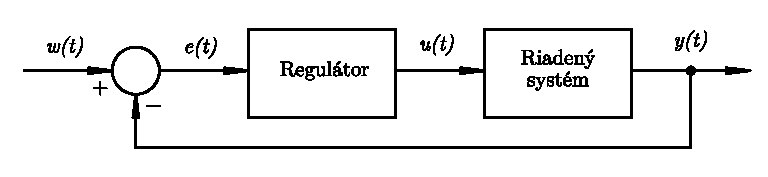
\includegraphics{schURO_regodch.pdf}
    \input{../fig_standalone/schURO_regodch.pdf_tex}
	}

	\figcaption{Uzavretý regulačný obvod s regulačnou odchýlkou a regulátorom.}
    \label{schURO_regodch.pdf}
    }

\end{center}

Je možné konštatovať, že na obr.~\ref{schURO_regodch.pdf} je celkový riadiaci systém tvorený dvomi prvkami: výpočtom regulačnej odchýlky a regulátorom. Typicky, vstupom regulátora je regulačná odchýlka.

Pre zdôraznenie faktu, že v uvedenom prípade ide jednoznačne (už z princípu informácie o odchýlke \eqref{regodch}) o zápornú spätnú väzbu môžeme kresliť schému nasledovne:

\begin{center}

    \vbox{%
    \makebox[\textwidth][c]{%
	% 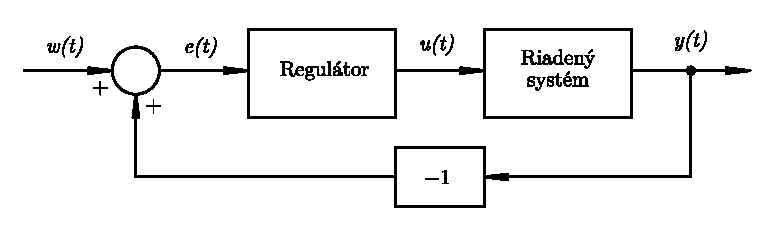
\includegraphics{schURO_regodchminus.pdf}
    \input{../fig_standalone/schURO_regodchminus.pdf_tex}
	}

    \vspace{-2mm}

	\figcaption{Uzavretý regulačný obvod s blokom vyjadrujúcim zápornú spätnú väzbu.}
	\label{schURO_regodchminus.pdf}
    }

\end{center}

\subsection{Lineárny uzavretý regulačný obvod}

V prípade, že riadiaci a riadený systém je možné opísať ako lineárne dynamické systémy, hovoríme o lineárnom uzavretom regulačnom obvode.

Typicky hovoríme, že regulátor, ktorého vstupom je regulačná odchýlka, a riadený systém je vtedy možné reprezentovať prenosovými funkciami. Klasický lineárny uzavretý regulačný obvod je potom možné schematicky znázorniť nasledovne:

\begin{center}

    \vbox{%
    \makebox[\textwidth][c]{%
	% 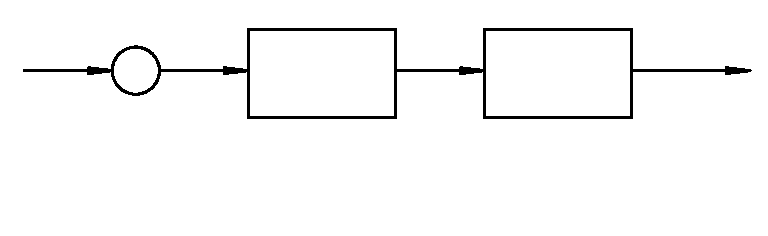
\includegraphics{schLinURO_basic.pdf}
    \input{../fig_standalone/schLinURO_basic.pdf_tex}
	}

    \vspace{-3mm}

	\figcaption{Lineárny uzavretý regulačný obvod.}
    \label{schLinURO_basic.pdf}
    }
	
\end{center}

V tomto prípade všetky bloky v schéme sú tvorené prenosovými funkciami (aj $-1$ je v princípe prenosová funkcia) pričom $G_R(s)$ je prenosová funkcia regulátora a  $G_S(s)$ je prenosová funkcia riadeného systému (hovorí sa tiež prenosová funkcia riadenej sústavy).

Avšak, ak sú blokmi URO prenosové funkcie, potom namiesto časových signálov je možné uvažovať ich Laplaceove obrazy (L-obrazy), teda $W(s)$, $E(s)$, $U(s)$ a $Y(s)$.



\subsubsection{Otvorený regulačný obvod}

S využitím algebry prenosových funkcií vidíme, že $G_R(s)$ a $G_S(s)$ sú v sérii a teda máme
\begin{align}
    G_{ORO}(s) = G_R(s) G_S(s)
\end{align}
pričom $G_{ORO}(s)$ je prenosová funkcia súvisiaca s pojmom \emph{otvorený regulačný obvod} -- je to situácia keď sa neuvažuje spätná väzba (obvod nie je uzavretý).

\begin{center}

    \vspace{-2mm}

    \vbox{%
    \makebox[\textwidth][c]{%
	% 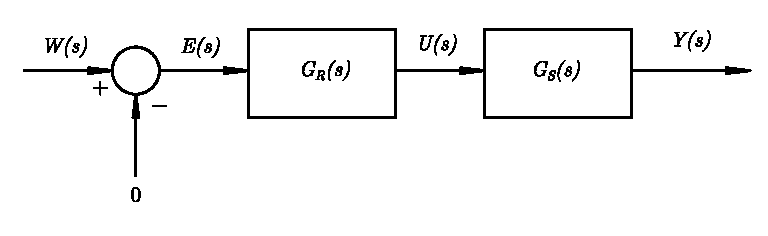
\includegraphics{schLinORO_basic.pdf}
    \input{../fig_standalone/schLinORO_basic.pdf_tex}    
	}

    \vspace{-3mm}

	\figcaption{Otvorený regulačný obvod.}
    \label{schLinORO_basic.pdf}
    }
	
\end{center}






\subsubsection{Prenosová funkcia URO}

Zároveň, na URO je potom jednoduché pozrieť sa ako na jeden celok. Celkovým výstupom URO je výstupná veličina $y(t)$, ktorej L-obraz je $Y(s)$, a celkovým vstupom URO je žiadaná hodnota $w(t)$ s obrazom $W(s)$. Pomer obrazov $W(s)$ a $Y(s)$ je prenosovou funkciou URO.
\begin{align}
    \frac{Y(s)}{W(s)} = G_{URO}(s)
\end{align}

Prenosovú funkciu URO je ďalej možné konkretizovať s využitím algebry prenosových funkcií. S využitím $G_{ORO}(s)$ máme situáciu:

\begin{center}

    \vspace{-1mm}

    \vbox{%
    \makebox[\textwidth][c]{%
	% 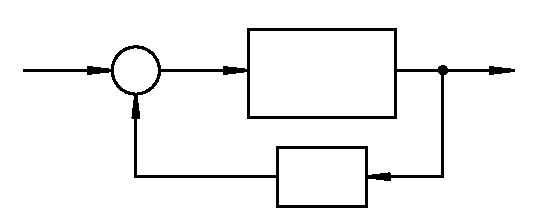
\includegraphics{schLinURO_basic_soro.pdf}
    \input{../fig_standalone/schLinURO_basic_soro.pdf_tex} 
	}

    \vspace{-1mm}

	\figcaption{}
    \label{schLinURO_basic_soro.pdf}
    }

\end{center}
a teda
\begin{align}
    G_{URO}(s) = \frac{G_{ORO}(s)}{1+G_{ORO}(s)} = \frac{G_R(s) G_S(s)}{1 + G_R(s) G_S(s)}
\end{align}
Tejto prenosovej funkcii sa tiež hovorí prenosová funkcia riadenia



\subsubsection{Iné prenosové funkcie v URO}

Obdobne je možné skúmať aj iné pomery L-obrazov signálov v uzavretom regulačnom obvode. Napríklad tzv. prenosová funkcia regulačnej odchýlky
\begin{align}
    \frac{E(s)}{W(s)} = G_E(s)
\end{align}
V tomto prípade teda:

\begin{center}

    \vbox{%
    \makebox[\textwidth][c]{%
	% 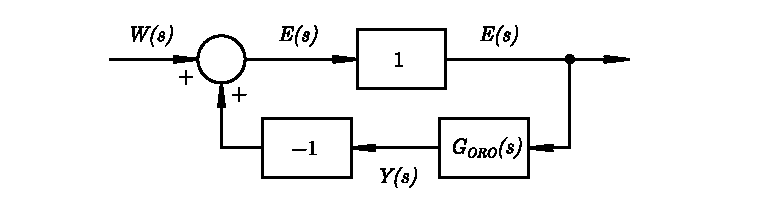
\includegraphics{schLinURO_GE.pdf}
    \input{../fig_standalone/schLinURO_GE.pdf_tex} 
	}

	\figcaption{}
    \label{schLinURO_GE.pdf}
    }

\end{center}
a
\begin{align}
    G_E(s) = \frac{1}{1+G_{ORO}(s)} = \frac{1}{1 + G_R(s) G_S(s)}
\end{align}

Túto skutočnosť je možné využiť pri skúmaní dynamiky a ustáleného stavu regulačnej odchýlky. Regulačná odchýlka totiž priamo hovorí o splnení či nesplnení cieľa riadenia.



Typickým je tiež uvažovať tzv. poruchu akčného zásahu a skúmať jej vplyv na výstup URO. Situácia vyzerá nasledovne:

\begin{center}

    \vbox{%
    \makebox[\textwidth][c]{%
	% 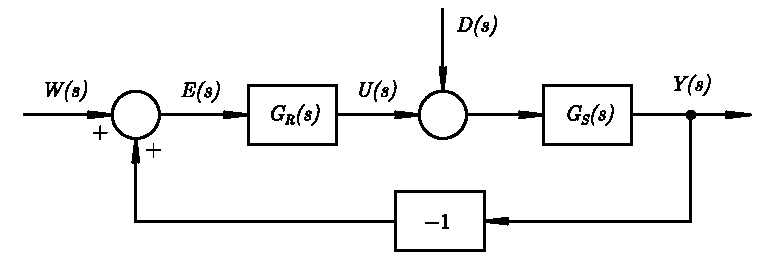
\includegraphics{schLinURO_basic_porucha.pdf}
    \input{../fig_standalone/schLinURO_basic_porucha.pdf_tex} 
	}

	\figcaption{Lineárny uzavretý regulačný obvod s uvažovaním poruchy akčného zásahu.}
    \label{schLinURO_basic_porucha.pdf}
    }
	
\end{center}


Pre izolovanie vplyvu poruchy na výstupnú veličinu je v prvom rade potrebné neuvažovať vplyv samotnej žiadanej hodnoty, teda $W(s) = 0$. Potom hovoríme o~prenosovej funkcii poruchy ak
\begin{align}
    \frac{Y(s)}{D(s)} = G_D(s)
\end{align}
teda:
\begin{center}

    \vbox{%
    \makebox[\textwidth][c]{%
	% 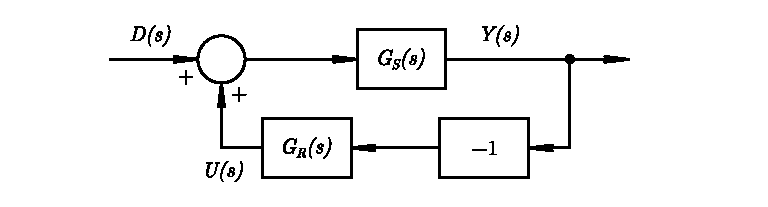
\includegraphics{schLinURO_GD.pdf}
    \input{../fig_standalone/schLinURO_GD.pdf_tex}
	}

	\figcaption{}
    \label{schLinURO_GD.pdf}
    }
	
\end{center}
a
\begin{align}
    G_D(s) = \frac{G_S(s)}{1 + G_S(s) G_R(s)}
\end{align}



\subsubsection{Stabilita URO}

Uvažuje sa tu o lineárnom URO a teda existuje prenosová funkcia URO. Akékoľvek otázky súvisiace so stabilitou URO sú preto totožné ako v prípade prenosovej funkcie vo všeobecnosti. Stabilita URO je daná charakteristickým polynómom prenosovej funkcie URO a teda polohou pólov URO v komplexnej rovine.





\subsubsection{Kvalita URO}

Pod kvalitou URO sa typicky rozumie presnosť sledovania zmien signálu $w(t)$ (žiadanej hodnoty) výstupnou veličinou $y(t)$. Ideálnym URO by bol taký, kde $y(t) = w(t) \  \forall t$, alebo teda $e(t) = w(t) - y(t) = 0  \  \forall t$.
Pre reálne systémy so zotrvačnosťou je to však nereálna požiadavka.

Je účelné vyšetrovať kvalitu URO (kvalitu riadenia) separátne v ustálenom stave a~v~prechodných stavoch (prechodných dejoch).

\paragraph{Kvalita v ustálenom stave}

Kritériom kvality v ustálenom stave je v princípe
\begin{align}
    \left| \lim_{t \to \infty} e(t) \right| = \left| e(\infty) \right| \to \min
\end{align}
kde
\begin{align}
    e(\infty) = w(\infty) - y(\infty)
\end{align}
sa nazýva trvalá regulačná odchýlka. V ideálnom prípade samozrejme $\left| e(\infty) \right| = 0$, t.j. $y(\infty) = w(\infty)$.


Typickými časovými priebehmi signálu $w(t)$ sú, zovšeobecnene povedané, skok polohy, skok rýchlosti a skok zrýchlenia. Všetky tieto prípady možno vyjadriť ako
\begin{align}
    w(t) = w_p \ t^q
\end{align}
kde $w_p$ je konštanta a $q$ nadobúda hodnoty $0$, $1$ alebo $2$. L-obrazom takéhoto signálu je
\begin{align}
    W(s) = \frac{q!}{s^{q+1}}w_p
\end{align}


Uvažujme všeobecne zapísanú prenosovú funkciu otvoreného regulačného obvodu:
\begin{align}
    G_{ORO}(s) = \frac{K}{s^\nu} \frac{b_m s^m + \ldots b_1 s + 1}{a_{n-\nu}s^{n-\nu} + \ldots + a_1s + 1}
\end{align}
kde $\nu$ rád astatizmu a $K$ je zosilnenie predmetnej prenosovej funkcie. Z prenosovej funkcie  regulačnej odchýlky potom máme
\begin{align}
\begin{aligned}
    E(s) &= \frac{W(s)}{1 + G_{ORO}(s)}
    \\&= \frac{s^\nu \left( a_{n-\nu}s^{n-\nu} + \ldots + a_1s + 1 \right)}{s^\nu \left( a_{n-\nu}s^{n-\nu} + \ldots + a_1s + 1 \right) + K \left( b_m s^m + \ldots b_1 s + 1 \right)}
    \frac{q!}{s^{q+1}}w_p
\end{aligned}
\end{align}
Na základe vety o konečnej hodnote platí
\begin{align}
    e(\infty) = \lim_{s\to 0} s E(s) =  \lim_{s\to 0} \left( q! w_p \frac{s^{\nu-q}}{s^\nu + K} \right)
\end{align}
Potom je zrejmé, že ak $\nu > q$ potom $e(\infty) = 0$. Ďalej ak $\nu < q$ potom $e(\infty) = \infty$ (a~teda URO je v~princípe nestabilný). Nakoniec ak $\nu = q$ potom $ 0 < e(\infty) < \infty$ a~teda vzniká nenulová trvalá regulačná odchýlka. Hodnotu trvalej regulačnej odchýlky je tiež možné aj vyjadriť, napríklad pre $\nu = q = 0$ je $e(\infty) = \frac{w_p}{1 + K}$.





\subsection{Návrh (lineárneho) URO vo všeobecnosti}

V princípe sa dajú klasifikovať tri typické východiskové situácie.

\begin{enumerate}[leftmargin=0pt, labelsep=4mm, itemsep=0pt]
    \item Je daná štruktúra riadiaceho systému a~navrhujú sa jeho parametre. \newline V tomto prípade to znamená, že poznáme stupne polynómov v~prenosovej funkcii $G_R(s)$ ale nepoznáme hodnoty koeficientov v~polynómoch, ktoré sú v~princípe parametrami riadiaceho systému ako celku.

    \item Navrhuje sa aj štruktúra (nie je presne daná) aj parametre. \newline Teda pri $G_R(s)$ aj stupne aj koeficienty polynómov.

    \item Štruktúra je čiastočne známa (napríklad relatívny stupeň $G_R(s)$) a pri týchto podmienkach sa následne navrhujú parametre.

\end{enumerate}

\noindent
Nástrojmi a informáciami využívanými pri návrhu sú:

\begin{itemize}[leftmargin=0pt, labelsep=4mm, itemsep=0pt]

    \item Požiadavky na kvalitu prechodného deja a ustáleného stavu regulačného obvodu.

    \item Vlastnosti a matematický model riadeného systému

    \item Časové priebehy výstupnej veličiny riadeného systému, typicky prechodové charakteristiky a podobne.

    \item Znalosť/odhad poruchových veličín, obmedzenia akčného zásahu a podobne\ldots
\end{itemize}




\section{O PID regulátore}

PID regulátor patrí medzi najviac rozšírené súčasti riadiacich systémov vo všeobecnosti.

V princípe využíva regulačnú odchýlku a tiež je ho možné opísať pomocou lineárneho dynamického systému a teda pomocou prenosovej funkcie.

Názov \emph{PID} regulátor vystihuje skutočnosť, že tento regulátor má tri principiálne zložky. Proporcionálnu, Integračnú a Derivačnú. Ide pri tom o tri spôsoby ako sa tu využíva informácia o regulačnej odchýlke.

Regulátor v skutočnosti pracuje s tromi signálmi. Prvým je samotná regulačná odchýlka $e(t) = w(t) - y(t)$. Z regulačnej odchýlky sa získavajú ďalšie dva signály. Časový integrál regulačnej odchýlky a časová derivácia regulačnej odchýlky. Formálnejšie
\begin{align}
    e_i(t) = \int e(t) \text{d}t
\end{align}
je časový integrál regulačnej odchýlky a
\begin{align}
    e_d(t) = \frac{\text{d}e(t)}{\text{d}t}
\end{align}
je časová derivácia regulačnej odchýlky.

Každý z týchto signálov je násobený (zosilnený) nejakou nastaviteľnou konštantou (parametrom regulátora) a výsledný akčný zásah $u(t)$ je súčet týchto troch členov, teda
\begin{align}
    u(t) = P e(t) + I  \int e(t) \text{d}t + D  \frac{\text{d}e(t)}{\text{d}t}
\end{align}
kde $P$, $I$ a $D$ sú parametre (konštanty, čísla, zosilnenia) regulátora.







\subsection{Prenosová funkcia PID regulátora}

Zo všeobecného hľadiska je vstupom regulátora regulačná odchýlka -- signál $e(t)$. Jeho L-obrazom je $E(s)$. Výstupom regulátora je akčný zásah, ktorého L-obrazom je $U(s)$. Prenosová funkcia PID regulátora potom formálne je
\begin{align}
    G_R(s) = \frac{U(s)}{E(s)}
\end{align}
alebo teda akčný zásah je
\begin{align}
    U(s) = G_R(s) E(s)
\end{align}

L-obrazom integrálu regulačnej odchýlky je $\frac{1}{s} E(s)$ a L-obrazom derivácie regulačnej odchýlky je $sE(s)$. Potom akčný zásah je
\begin{align}
    U(s) = P E(s) + I  \frac{1}{s} E(s) + D  sE(s)
\end{align}
konvenčne sa v~tejto súvislosti pre označenie parametrov PID používajú $r_0$, $r_{-1}$ a~$r_1$, kde číselný index má vyjadrovať mocninu premennej $s$, pri ktorej sa parameter nachádza. Teda
\begin{align}
    U(s) = r_0 E(s) + r_{-1}  \frac{1}{s} E(s) + r_1  sE(s)
\end{align}

Prenosová funkcia PID regulátora je potom v tvare
\begin{align} \label{tfPID}
    G_R(s) = r_0  + r_{-1}  \frac{1}{s}  + r_1  s
\end{align}
Tento tvar sa nazýva zložkový tvar, totiž, túto prenosovú funkciu je možné vyjadriť aj v tvare
\begin{align}
    G_R(s) = P \left( 1 +  \frac{1}{T_I s}  +  T_D  s \right)
\end{align}
kde zmyslom je zavedenie časových konštánt $T_I$ a $T_D$ (tieto parametre majú rozmer času) a pri tom platí $P = r_0$, $T_I = \frac{r_0}{r_{-1}}$ a $T_I = \frac{r_1}{r_0}$.

Len pre názornosť, ak by sme chceli vyjadriť prenosovú funkciu \eqref{tfPID} ako jediný zlomok, potom
\begin{align} \label{tfPID2}
    G_R(s) =  \frac{ r_1 s^2 + r_0 s + r_{-1} }{s}
\end{align}
kde je zrejmé, že stupeň čitateľa je vyšší ako stupeň menovateľa a teda ide o~nekauzálny systém. To súvisí so skutočnosťou, že realizovať časovú deriváciu, takú, pri ktorej by bola veľkosť časového úseku $\text{d}t$ nekonečne malá, je nereálne. V praxi je možné realizovať kvalitnú aproximáciu ideálnej časovej derivácie, čo sa v týchto súvislostiach prejaví tak, že obrazom signálu v derivačnej zložke nie je $sE(s)$, ale iný výraz, taký, že to má za následok splnenie podmienky kauzality v celkovej prenosovej funkcii PID regulátora.









\subsection{Bloková schéma PID regulátora}

Schematicky, pomocou základných funkčných prvkov, vzhľadom na jeho prenosovú funkciu, je možné PID regulátor znázorniť nasledovne:

\begin{center}

    \vspace{-1mm}

    \vbox{%
    \makebox[\textwidth][c]{%
	% 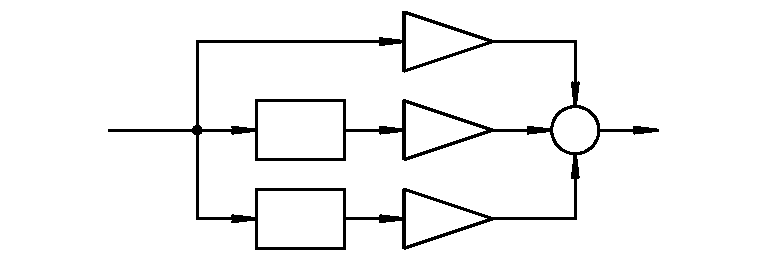
\includegraphics{PID_blokSch.pdf}
    \input{../fig_standalone/PID_blokSch.pdf_tex}
	}

    \vspace{-3mm}

	\figcaption{Bloková schéma PID regulátora}
    \label{PID_blokSch.pdf}
    }

    \vspace{-1mm}

\end{center}






\section{O výbere štruktúry PID regulátora}

PID regulátor vo všeobecnosti pozostáva z troch zložiek. Často však nie je potrebné použiť všetky tri zložky. Niekedy to môže byť až výslovne nežiadúce.

V princípe je možné uvažovať tri samostatné regulátory (zložky PID regulátora). Hovoríme o P-regulátore (využíva sa len proporcionálna zložka PID), o I-regulátore (využíva sa len integračná zložka PID) a o D-regulátore (využíva sa len derivačná zložka PID).

Zároveň je možné uvažovať aj vzájomné kombinácie uvedených regulátorov. Veľmi častým prípadom je PI regulátor. Aj PD regulátor je v praxi používaný. Niečo ako „ID regulátor“ môže mať uplatnenie ale ide o ojedinelé prípady.




\subsection{Príklady}


\subsubsection{P regulátor a SS1R}

Majme URO, kde
\begin{align}
    G_R(s) = r_0 \qquad \text{a} \qquad  G_S(s) = \frac{K}{Ts+1}
\end{align}
teda:

\begin{center}

    \vbox{%
    \makebox[\textwidth][c]{%
    \input{../fig_standalone/URO_P_SS1R.pdf_tex}
    }

	\figcaption{}
    \label{URO_P_SS1R}
    }
	
\end{center}




\paragraph{Prenosová funkcia ORO}
Nájdime prenosovú funkciu ORO.
\begin{align}
    G_{ORO}(s) = G_R(s) G_S(s) = \frac{r_0 K}{Ts+1}
\end{align}


\paragraph{Prenosová funkcia URO}
Nájdime prenosovú funkciu URO.
\begin{equation}
\begin{aligned}
    G_{URO}(s)
    &=  \frac{G_{ORO}(s)}{1+G_{ORO}(s)}
    = \cfrac{\cfrac{r_0 K}{Ts+1}}{1+\cfrac{r_0 K}{Ts+1}}
    = \frac{\cfrac{r_0 K}{Ts+1}}{\cfrac{Ts+1 + r_0 K}{Ts+1}}
    \\&= \frac{r_0 K}{Ts+ (1 + r_0 K)}
    = \frac{ \cfrac{r_0 K}{T}}{s+ \cfrac{1 + r_0 K}{T}}
\end{aligned}
\end{equation}
URO je systémom prvého rádu bez astatizmu.


\paragraph{Stabilita}
Vyšetrime stabilitu URO. Charakteristický polynóm URO je
\begin{align}
    A(s) = s + \frac{1 + r_0 K}{T}
\end{align}
Pól URO je $s_1 = - \frac{1 + r_0 K}{T}$. URO je stabilný ak $\Re\{ s_1 \} < 0$.




\paragraph{Kvalita v ustálenom stave}
Uvažujme $w(t) = 1$ a vyšetrime veľkosť trvalej regulačnej odchýlky $e(\infty)$.

L-obrazom žiadanej hodnoty je $W(s) = \frac{1}{s}$. Teda
\begin{align}
    Y(s) = G_{URO}(s) \frac{1}{s}
\end{align}
Podľa vety o konečnej hodnote platí
\begin{align}
    y(\infty) = \lim_{s\to 0} s Y(s) = \lim_{s\to 0} \left( \ s \ G_{URO}(s) \ \frac{1}{s} \right)
\end{align}
takže ak uvažujeme $w(t) = 1$, potom
\begin{align}
    y(\infty) =  \lim_{s\to 0} \ G_{URO}(s)
\end{align}
V tomto prípade
\begin{align}
    y(\infty)
    =  \lim_{s\to 0} \left(  \frac{r_0 K}{Ts+ (1 + r_0 K)} \right)
    =  \frac{r_0 K}{(1 + r_0 K)}
\end{align}
Trvalá regulačná odchýlka je $e(\infty) = w(\infty) - y(\infty)$, pričom v tomto prípade samozrejme $ w(\infty) = 1$, teda
\begin{align}
    e(\infty)
    = w(\infty) - y(\infty)
    = 1 -  \frac{r_0 K}{(1 + r_0 K)}
    =\frac{1 + r_0 K - r_0 K}{(1 + r_0 K)}
    =\frac{1}{(1 + r_0 K)}
\end{align}
Trvalá regulačná odchýlka bude vždy nenulová.




\paragraph{Prechodný dej}
V tomto prípade URO opisuje prenosová funkcia 1. rádu. Tým je daný aj typický tvar prechodovej charakteristiky URO (tri prípady: kladný/záporný/nulový pól). Zároveň tu má význam hovoriť o časovej konštante URO, ktorá má hodnotu $\frac{T}{(1 + r_0 K)}$ a zosilnení URO, ktoré má hodnotu $\frac{r_0 K}{(1 + r_0 K)}$.







\paragraph{Simulácia}

Pre príklad uvažujme $K = 1$, $T = 1$ a parameter $r_0 = 1$. Výsledok simulácie je nasledovný:


\begin{center}

    \vbox{%
    \makebox[\textwidth][c]{%
    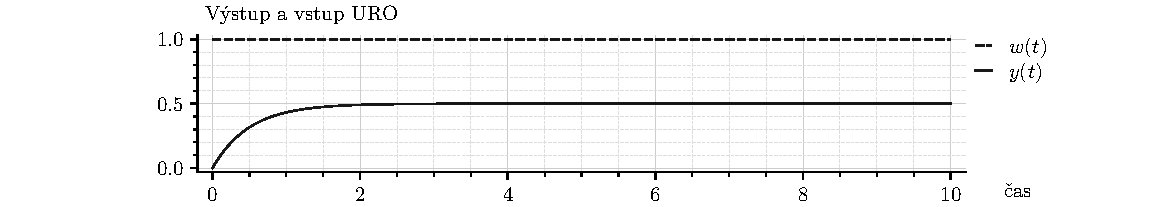
\includegraphics{MRS10_prikl_01a_panel_wy.pdf}
    }

    \makebox[\textwidth][c]{%
    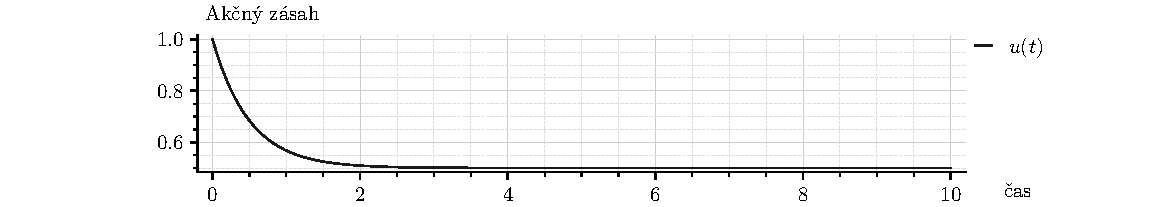
\includegraphics{MRS10_prikl_01a_panel_u.pdf}
    }

    \figcaption{}
    }

\end{center}

\noindent
Pre ilustráciu, regulačná odchýlka:


\begin{center}

    \vbox{%
    \makebox[\textwidth][c]{%
    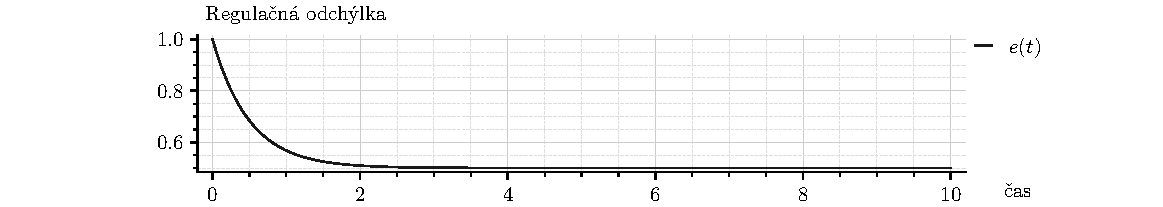
\includegraphics{MRS10_prikl_01a_panel_e_log.pdf}
    }

    % \makebox[\textwidth][c]{%
    % 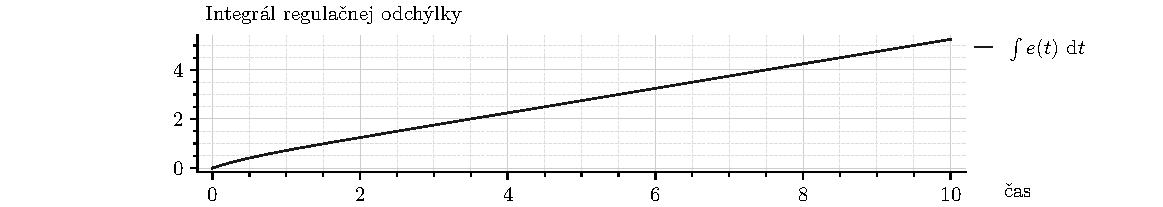
\includegraphics{MRS11_prikl_01a_panel_int_e_log.pdf}
    % }
    
    % \makebox[\textwidth][c]{%
    % 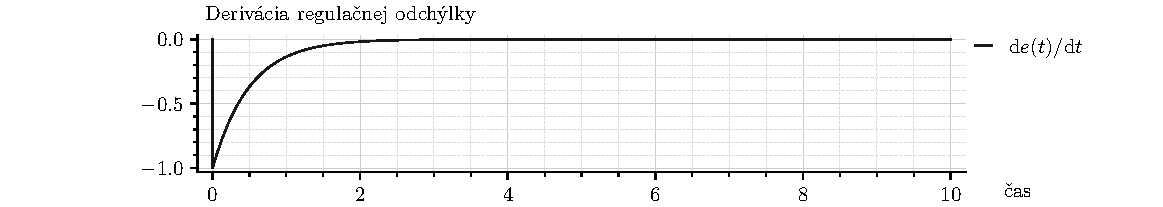
\includegraphics{MRS11_prikl_01a_panel_der_e_log.pdf}
    % }

    \figcaption{}
    }

\end{center}













\subsubsection{PI regulátor a SS1R}

Majme URO, kde
\begin{align}
    G_R(s) = r_0 + \frac{r_{-1}}{s} \qquad \text{a} \qquad  G_S(s) = \frac{K}{Ts+1}
\end{align}
teda:

\begin{center}

    \vbox{%
    \makebox[\textwidth][c]{%
    \input{../fig_standalone/URO_PI_SS1R.pdf_tex}
    }

	\figcaption{}
	\label{URO_PI_SS1R}
    }

\end{center}

\paragraph{Prenosová funkcia ORO}
Nájdime prenosovú funkciu ORO.
\begin{align}
    G_{ORO}(s) = G_R(s) G_S(s) =  \frac{K r_0 s + Kr_{-1}}{Ts^2+s}
\end{align}

\paragraph{Prenosová funkcia URO}
Nájdime prenosovú funkciu URO.
\begin{align}
    \begin{aligned}
    G_{URO}(s)
    &=  \frac{G_{ORO}(s)}{1+G_{ORO}(s)}
    = \frac{   \cfrac{K r_0 s + Kr_{-1}}{Ts^2+s}   }{   1+  \cfrac{K r_0 s + Kr_{-1}}{Ts^2+s} }
    = \frac{   \cfrac{K r_0 s + Kr_{-1}}{Ts^2+s}   }{   \cfrac{Ts^2+s + K r_0 s + Kr_{-1}}{Ts^2+s} } \\
    &= \frac{   \cfrac{K r_0 s + Kr_{-1}}{Ts^2+s}   }{   \cfrac{Ts^2+  (1 + K r_0) s + Kr_{-1}}{Ts^2+s} }
    = \frac{   K r_0 s + Kr_{-1}   }{   Ts^2+  (1 + K r_0) s + Kr_{-1} }
    \end{aligned}
\end{align}
URO je systémom druhého rádu bez astatizmu s jednou nulou.



\paragraph{Stabilita}

Vyšetrime stabilitu URO. Charakteristický polynóm URO je
\begin{align}
    A(s) = Ts^2+  (1 + K r_0) s + Kr_{-1}
\end{align}
Zaujímajú nás podmienky, pri ktorých bude URO stabilný. Tieto podmienky ba malo byť možné využiť pri návrhu/voľbe parametrov regulátora. Využime skutočnosť, že ak sú všetky koeficienty polynómu druhého stupňa kladné, potom jeho korene majú zápornú reálnu časť.

URO bude teda stabilný ak
\begin{align}
    T>0 \qquad 1+K r_0 >0 \qquad K r_{-1} > 0
\end{align}



\paragraph{Kvalita v ustálenom stave}
Uvažujme $w(t) = 1$ a vyšetrime veľkosť trvalej regulačnej odchýlky $e(\infty)$.

Cieľom je zistiť aká je dosiahnuteľná minimálna trvalá regulačná odchýlka, teda  $e(\infty) = w(\infty) - y(\infty)$.

Keďže $W(s) = \frac{1}{s}$ a URO je stabilný, potom
\begin{align}
    y(\infty) = \lim_{s\to0} G_{URO}(s) = \frac{K r_{-1}}{K r_{-1}} = 1
\end{align}
Trvalá regulačná odchýlka je $e(\infty) = w(\infty) - y(\infty)$, pričom v tomto prípade samozrejme $ w(\infty) = 1$, teda
\begin{align}
    e(\infty)
    = w(\infty) - y(\infty)
    = 1 - 1
    = 0
\end{align}
Trvalá regulačná odchýlka bude vždy nulová.



\paragraph{Prechodný dej}
Cieľom je vyhodnotiť možnosti ovplyvnenia prechodného deja, ktorý vykazuje URO, pomocou parametrov regulátora.

V tomto prípade je prenosová funkcia URO prenosovou funkciou druhého rádu. Prechodný dej teda môže byť kmitavý (dva komplexne združené póly) alebo aperiodický (dva reálne póly).

Charakteristický polynóm v tomto prípade je
\begin{align}
    A(s)  =  Ts^2+  (1 + K r_0) s + Kr_{-1}
\end{align}
a jeho korene
\begin{align}
    s_{1,2} = \frac{-(1+K r_0)}{2T} \pm \frac{ \sqrt{(1+K r_0)^2 - 4TKr_{-1} }}{2T}
\end{align}
O charaktere koreňov rozhoduje diskriminant, teda v tomto prípade ak
\begin{align}
     (1+K r_0)^2 - 4TKr_{-1} \geq 0
\end{align}
tak prechodný dej URO bude aperiodický, inak bude kmitavý.





\paragraph{Simulácia 1 (nekmitavý prechodný dej)}

Pre príklad uvažujme $K = 1$, $T = 10$ a $r_0 = 15$, $r_{-1} = 1$. Výsledok je nasledovný:

% \vfill

\begin{center}

    \vbox{%
    \makebox[\textwidth][c]{%
    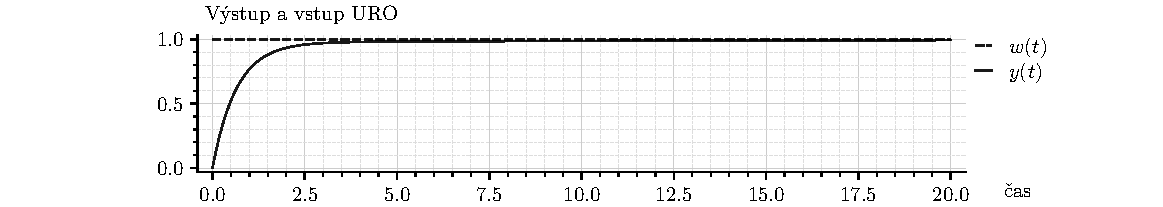
\includegraphics{MRS10_prikl_02a_panel_wy.pdf}
    }

    \makebox[\textwidth][c]{%
    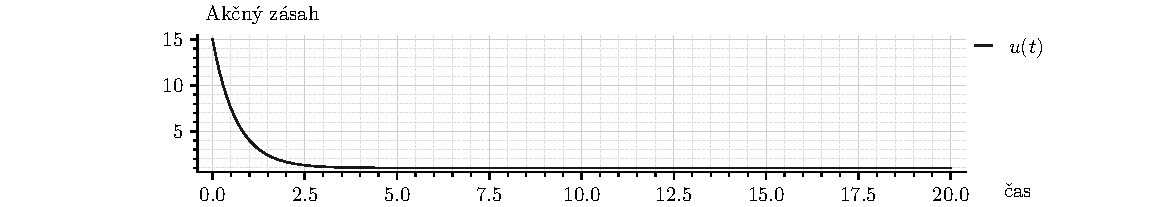
\includegraphics{MRS10_prikl_02a_panel_u.pdf}
    }

    \figcaption{}
    }

\end{center}

% \vfill

\noindent
Pre ilustráciu, regulačná odchýlka:

% \vfill

\begin{center}

    \vbox{%
    \makebox[\textwidth][c]{%
    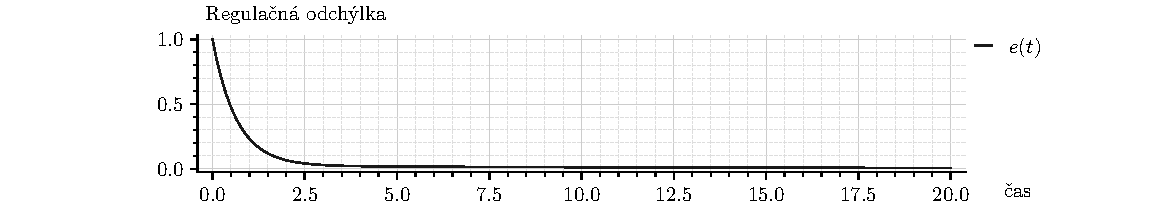
\includegraphics{MRS10_prikl_02a_panel_e_log.pdf}
    }

    \makebox[\textwidth][c]{%
    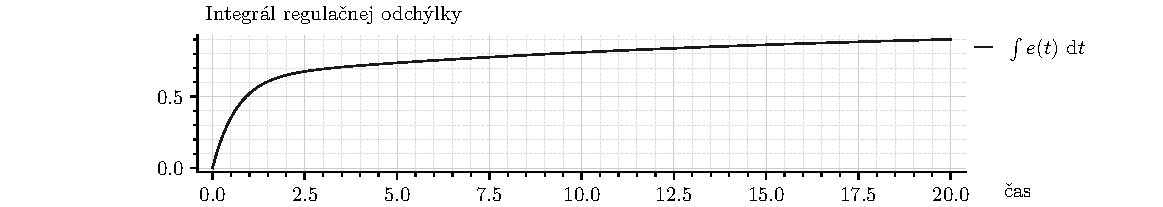
\includegraphics{MRS10_prikl_02a_panel_int_e_log.pdf}
    }
    %
    % \makebox[\textwidth][c]{%
    % 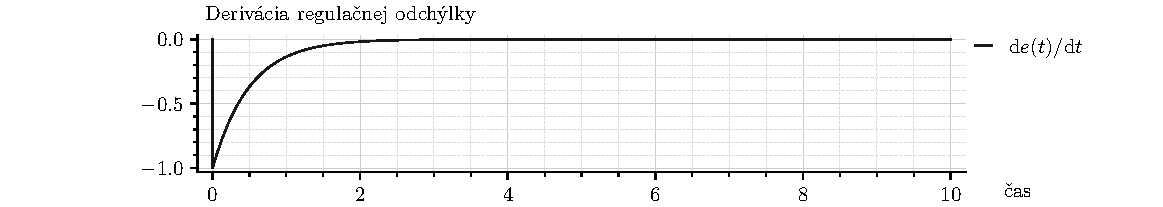
\includegraphics{MRS11_prikl_01a_panel_der_e_log.pdf}
    % }

    \figcaption{}
    }

\end{center}





\paragraph{Simulácia 2 (kmitavý prechodný dej)}

Pre príklad uvažujme $K = 1$, $T = 10$ a $r_0 = 2$, $r_{-1} = 0,5$. Výsledok je nasledovný:

% \vfill

\begin{center}

    \vbox{%
    \makebox[\textwidth][c]{%
    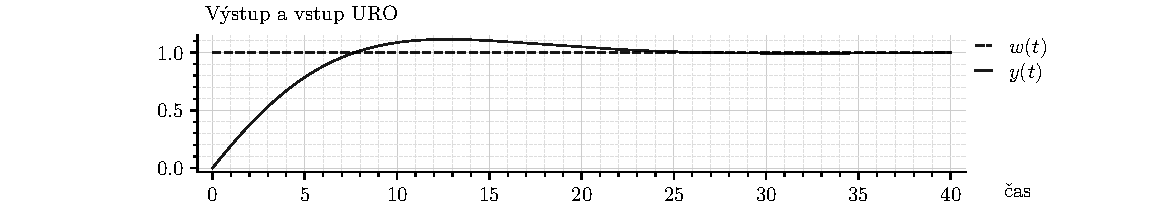
\includegraphics{MRS10_prikl_02b_panel_wy.pdf}
    }

    \makebox[\textwidth][c]{%
    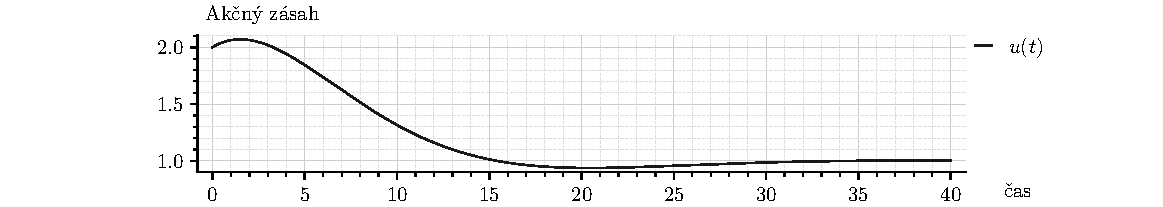
\includegraphics{MRS10_prikl_02b_panel_u.pdf}
    }

    \figcaption{}
    }

\end{center}



\noindent
Pre ilustráciu, regulačná odchýlka:

% \vfill

\begin{center}

    \vbox{%
    \makebox[\textwidth][c]{%
    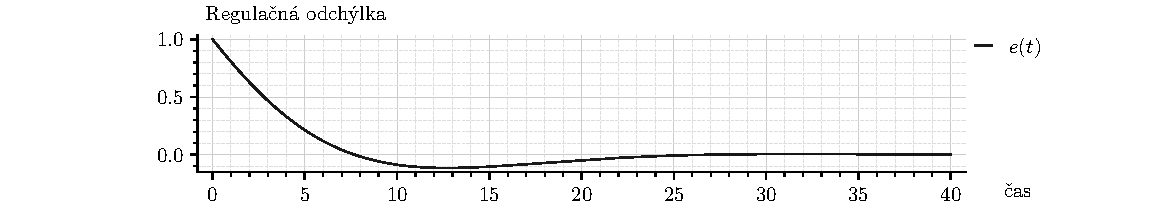
\includegraphics{MRS10_prikl_02b_panel_e_log.pdf}
    }

    \makebox[\textwidth][c]{%
    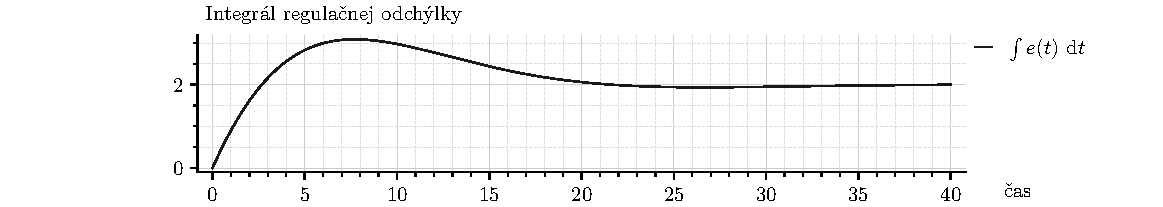
\includegraphics{MRS10_prikl_02b_panel_int_e_log.pdf}
    }
    %
    % \makebox[\textwidth][c]{%
    % 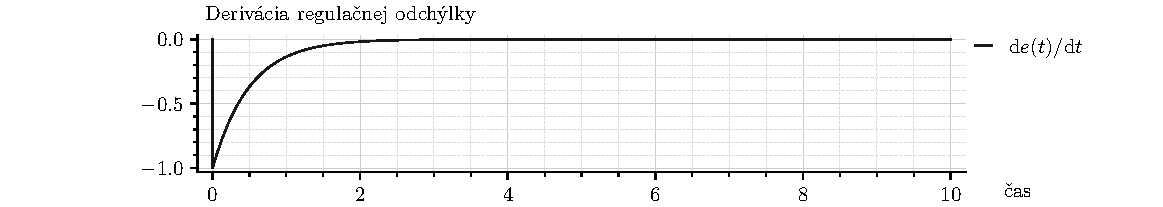
\includegraphics{MRS11_prikl_01a_panel_der_e_log.pdf}
    % }

    \figcaption{}
    }

\end{center}








\subsubsection{PI regulátor a AS1R}

Majme URO, kde
\begin{align}
    G_R(s) = r_0 + \frac{r_{-1}}{s} \qquad \text{a} \qquad  G_S(s) = \frac{1}{s}
\end{align}
teda:

\begin{center}

    \vbox{%
    \makebox[\textwidth][c]{%
    \input{../fig_standalone/URO_PI_AS1R.pdf_tex}
    }

	\figcaption{}
    \label{URO_PI_AS1R}
    }
	
\end{center}





\paragraph{Prenosová funkcia ORO}
Nájdime prenosovú funkciu ORO.
\begin{align}
    G_{ORO}(s) = G_R(s) G_S(s) =  \frac{r_0 s + r_{-1}}{s^2}
\end{align}


\paragraph{Prenosová funkcia URO}
Nájdime prenosovú funkciu URO.
\begin{align}
    \begin{aligned}
    G_{URO}(s)
    &=  \frac{G_{ORO}(s)}{1+G_{ORO}(s)}
    = \frac{   \cfrac{r_0 s + r_{-1}}{s^2}   }{     \cfrac{s^2 + r_0 s + r_{-1}}{s^2}   }
    = \frac{  r_0 s + r_{-1}   }{    s^2 + r_0 s + r_{-1}   }
    \end{aligned}
\end{align}
URO je systémom druhého rádu bez astatizmu s jednou nulou.

\paragraph{Stabilita}
Vyšetrime stabilitu URO. Charakteristický polynóm URO je
\begin{align}
    A(s) =  s^2 + r_0 s + r_{-1}
\end{align}
Nutnou a postačujúcou podmienkou stability teda je ak sú oba parametre regulátora kladné, $r_0 > 0$, $r_{-1} > 0$.

\paragraph{Kvalita v ustálenom stave}
Uvažujme $w(t) = 1$ a vyšetrime veľkosť trvalej regulačnej odchýlky $e(\infty)$. Keďže $W(s) = \frac{1}{s}$ (a URO je stabilný), potom
\begin{align}
    y(\infty) = \lim_{s\to0} G_{URO}(s) = \frac{r_{-1}}{r_{-1}} = 1
\end{align}
teda
\begin{align}
    e(\infty)
    = w(\infty) - y(\infty)
    = 1 - 1
    = 0
\end{align}
Trvalá regulačná odchýlka bude vždy nulová.

\paragraph{Prechodný dej}
Je závislý od pólov URO. Póly URO sú
\begin{align}
    s_{1,2} = \frac{-(r_0)}{2} \pm \frac{ \sqrt{r_0^2 - 4r_{-1} }}{T}
\end{align}
Ak teda
\begin{align}
     r_0^2 - 4r_{-1} \geq 0
\end{align}
prechodný dej bude aperiodický, inak bude kmitavý.







\paragraph{Simulácia 1 (nekmitavý prechodný dej)}

Pre príklad uvažujme $r_0 = 10$, $r_{-1} = 1$. Vtedy jednoznačne platí $r_0^2 - 4r_{-1} \geq 0$. Výsledok je nasledovný:

\begin{center}

    \vbox{%
    \makebox[\textwidth][c]{%
    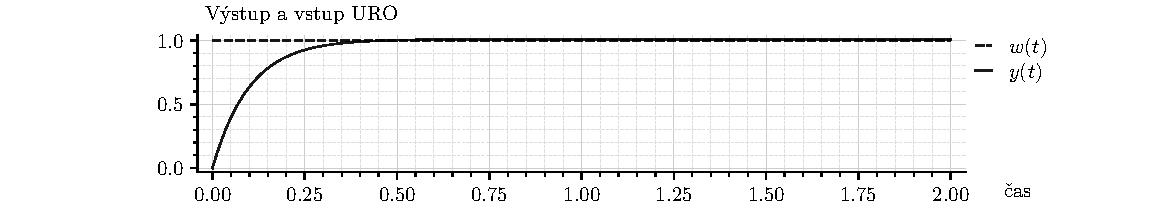
\includegraphics{MRS10_prikl_03a_panel_wy.pdf}
    }

    \makebox[\textwidth][c]{%
    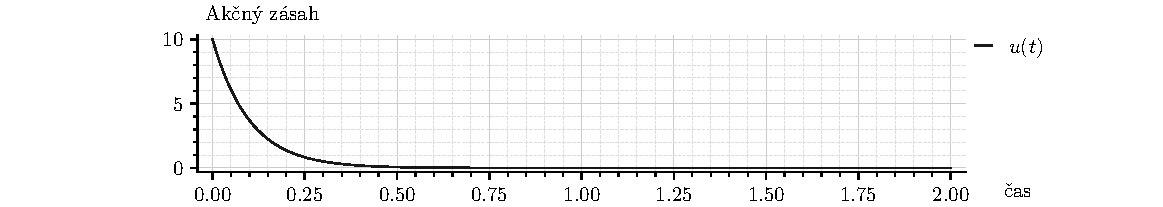
\includegraphics{MRS10_prikl_03a_panel_u.pdf}
    }

    % \makebox[\textwidth][c]{%
    % 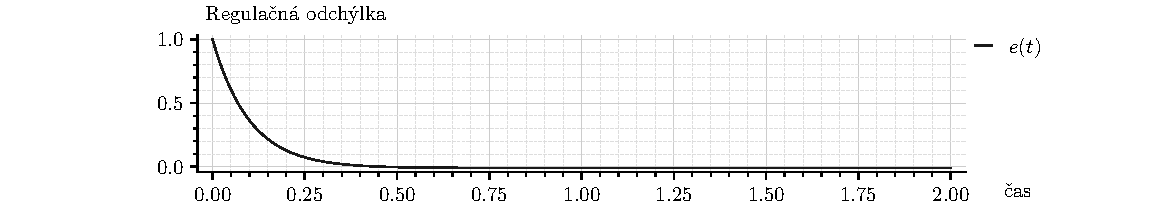
\includegraphics{MRS11_prikl_03a_panel_e_log.pdf}
    % }
    %
    % \makebox[\textwidth][c]{%
    % 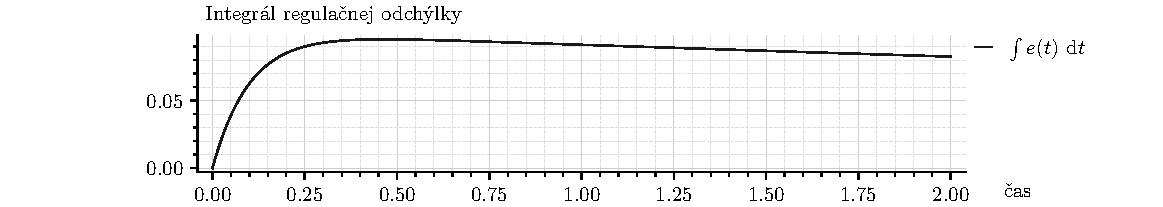
\includegraphics{MRS11_prikl_03a_panel_int_e_log.pdf}
    % }

    \figcaption{}
    }

\end{center}








\paragraph{Simulácia 2 (dva reálne póly)}

Pre príklad uvažujme $r_0 = 2$, $r_{-1} = 1$. Vtedy stále platí, že $r_0^2 - 4r_{-1} \geq 0$. Výsledok je však nasledovný, prejavuje sa vplyv nuly prenosovej funkcie URO na prechodovú charakteristiku URO.



\begin{center}

    \vbox{%
    \makebox[\textwidth][c]{%
    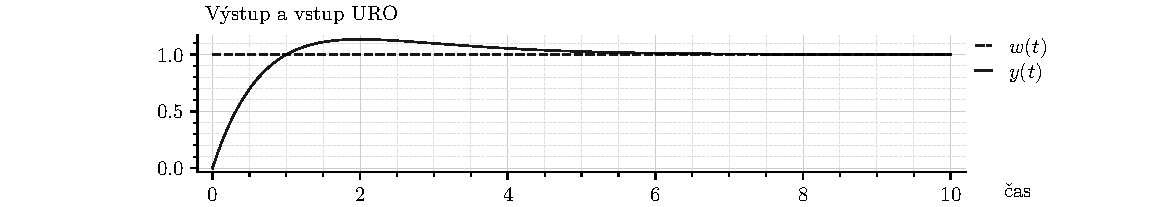
\includegraphics{MRS10_prikl_03b_panel_wy.pdf}
    }

    \makebox[\textwidth][c]{%
    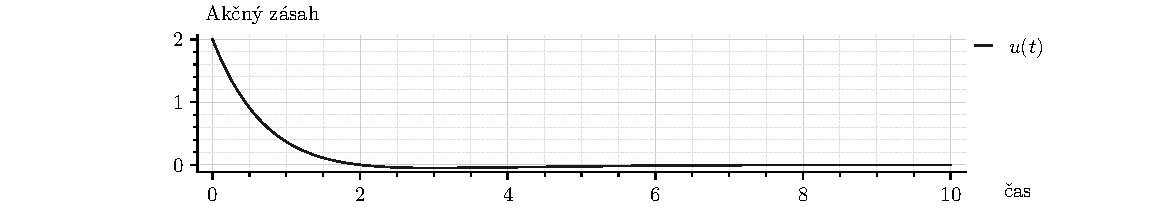
\includegraphics{MRS10_prikl_03b_panel_u.pdf}
    }

    % \makebox[\textwidth][c]{%
    % 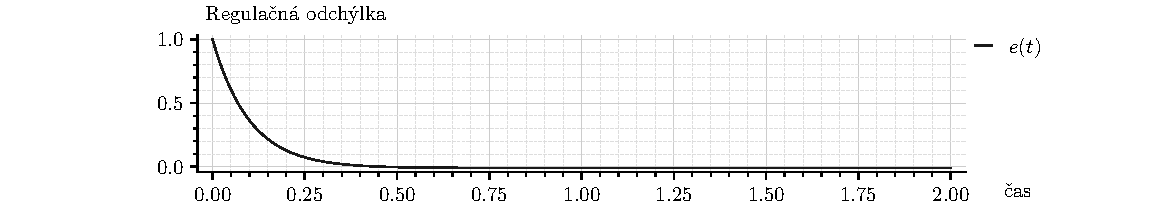
\includegraphics{MRS11_prikl_03a_panel_e_log.pdf}
    % }
    %
    % \makebox[\textwidth][c]{%
    % 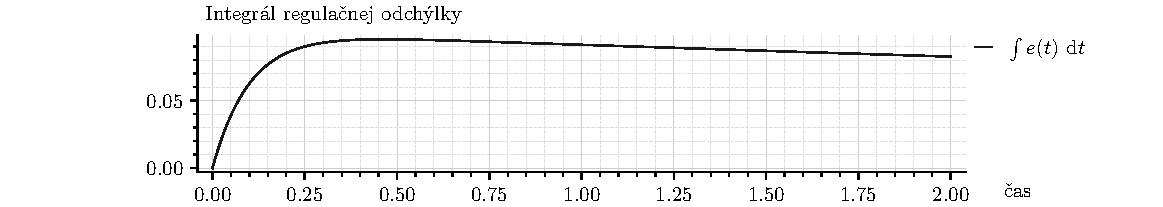
\includegraphics{MRS11_prikl_03a_panel_int_e_log.pdf}
    % }

    \figcaption{}
    }

\end{center}










\paragraph{Simulácia 3 (dva komplexne združené póly)}

Pre príklad uvažujme $r_0 = 0.5$, $r_{-1} = 1$. Vtedy  platí, že $r_0^2 - 4r_{-1} < 0$. Výsledok je nasledovný:


\begin{center}

    \vbox{%
    \makebox[\textwidth][c]{%
    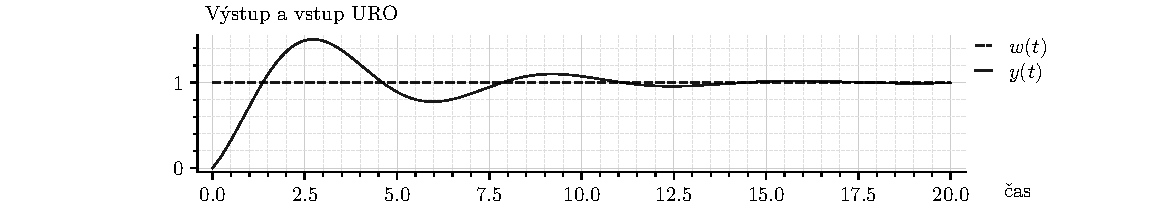
\includegraphics{MRS10_prikl_03c_panel_wy.pdf}
    }

    \makebox[\textwidth][c]{%
    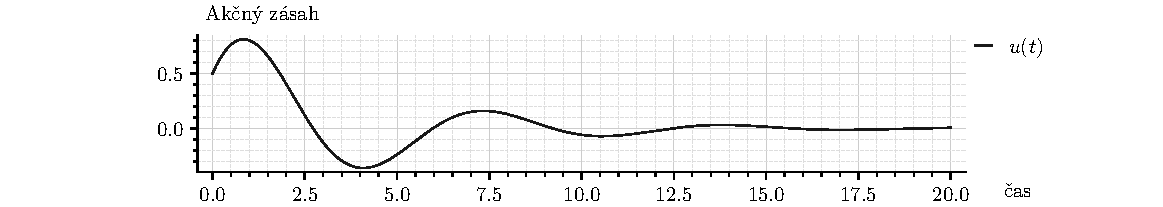
\includegraphics{MRS10_prikl_03c_panel_u.pdf}
    }

    % \makebox[\textwidth][c]{%
    % 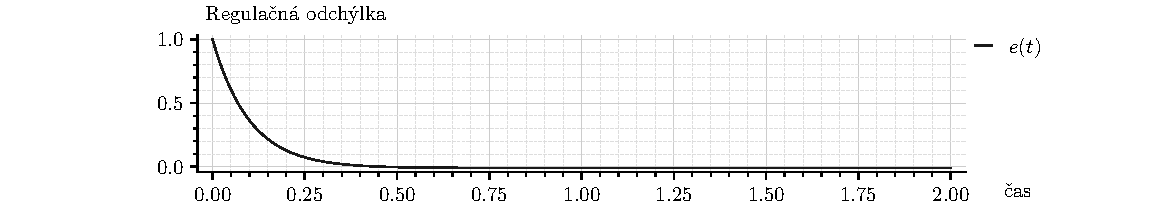
\includegraphics{MRS11_prikl_03a_panel_e_log.pdf}
    % }
    %
    % \makebox[\textwidth][c]{%
    % 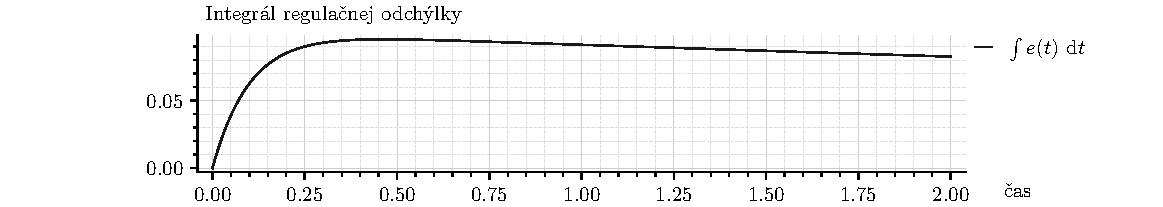
\includegraphics{MRS11_prikl_03a_panel_int_e_log.pdf}
    % }

    \figcaption{}
    }

\end{center}
















\section[O metódach návrhu PID regulátora]{O (vybraných) metódach návrhu PID regulátora}

Cieľom tohto textu je veľmi stručný úvod do metód návrhu parametrov PID regulátora v zmysle klasického lineárneho regulačného obvodu (URO) aký bol diskutovaný v~predchádzajúcom učebnom texte. Je teda zrejmé, že tieto metódy predpokladajú dostupnosť modelu riadeného systému vo forme prenosovej funkcie. Zvyčajne je tiež potrebné doplniť výstupy a výsledky metód o analýzu z hľadiska stability a kvality výsledného URO.


\subsection{Analytický opis URO ako východisko}

Metódy, ktorými sa tu budeme zaoberať, využívajú analytický opis URO ako východisko. Preto táto časť v skratke pripomína lineárny URO ako taký.

Ak totiž máme k dispozícii analytický opis URO, vieme o URO povedať prakticky čokoľvek. Vrátane toho ako má a môže vyzerať prenosová funkcia samotného regulátora v URO. 

Možných je relatívne veľa metód ako z matematického opisu URO odvodiť samotný regulátor a určiť jeho parametre. Napríklad sa môžeme priamo z~analytického opisu URO pokúsiť vyjadriť prenosovú funkciu regulátora (pozri časť~\ref{Číro analytické zamyslenie sa}). Celkom prirodzenou požiadavkou na URO môže byť stanovenie želanej dynamiky URO, čo v lineárnom URO vlastne znamená stanovenie polohy pólov URO (pozri časť~\ref{Metóda rozmiestňovania pólov}). Zmienené postupy sú na prvý pohľad jednouché avšak pri ich uplatňovaní sa nezriedkavo vyskytnú rôzne problémy, ktoré môžu viesť až k nemožnosti navrhnúť parametre regulátora tak aby bol daný cieľ riadenia splnený. Aj preto má význam skúmať metódy, ktoré na prvý pohľad nemusia byť zrejmé, avšak ich uplatnenie vedie k uspokojivým výsledkom v relatívne širšej triede úloh oproti zmieneným postupom. Príkladom takej dobre známej metódy je tu Metóda optimálneho modulu prezentovaná v časti~\ref{Metóda optimálneho modulu}.


V nasledujúcich častiach sú uvedené náznaky metód (relatívne jednoduchých) návrhu parametrov PID (alebo PI, P atď.). Tento učebný text však neskúma uvedené metódy vo všeobecnosti, neskúma možnosti a obmedzenia ich uplatnenia. Pre ďalšie štúdium sa čitateľ odkazuje na klasickú literatúru venovanú návrhu PID regulátorov (nespočetne veľa autorov a diel).




\paragraph{Klasický lineárny uzavretý regulačný obvod}

Pripomeňme, že uvažujeme klasický lineárny uzavretý regulačný obvod, ktorý je možné schematicky znázorniť nasledovne:

\begin{center}

    \vbox{%
    \makebox[\textwidth][c]{%
	% 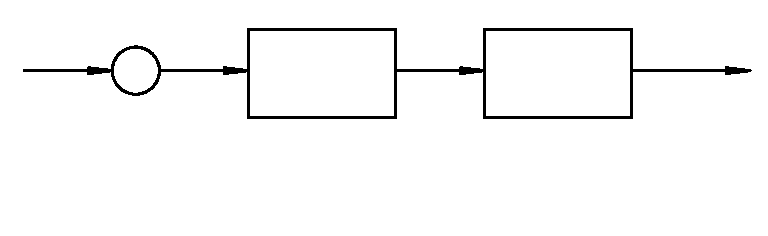
\includegraphics{schLinURO_basic.pdf}
    \input{../fig_standalone/schLinURO_basic.pdf_tex}
	}

    \vspace{-3mm}

	\figcaption{Lineárny uzavretý regulačný obvod.}
    \label{schLinURO_basic_2.pdf}
    }
	
\end{center}
V schéme $G_R(s)$ je prenosová funkcia regulátora a $G_S(s)$ je prenosová funkcia riadeného systému. Blokmi URO sú tu teda prenosové funkcie, potom namiesto časových signálov je možné uvažovať ich Laplaceove obrazy (L-obrazy), a teda $W(s)$ je želaná hodnota (setpoint), $E(s)$ je regulačná odchýlka, $U(s)$ je akčný zásah a $Y(s)$ je výstupná (riadená) veličina URO.



\paragraph{Prenosová funkcia ORO a URO}

Prenosové funkcie $G_R(s)$ a $G_S(s)$ sú v sérii a tvoria otvorený regulačný obvod, ktorého prenosová funkcia je v tvare
\begin{align}
    G_{ORO}(s) = G_R(s) G_S(s)
\end{align}

Celkovým výstupom URO je výstupná veličina $Y(s)$, a celkovým vstupom URO je žiadaná hodnota $W(s)$. Pomer obrazov $W(s)$ a $Y(s)$ je prenosovou funkciou URO.
\begin{align}
    \frac{Y(s)}{W(s)} = G_{URO}(s)
\end{align}
Konkrétne pre tu uvažovaný prípad a vzhľadom na vyššie uvedené
\begin{align} \label{defGURO}
    G_{URO}(s) = \frac{G_{ORO}(s)}{1+G_{ORO}(s)} = \frac{G_R(s) G_S(s)}{1 + G_R(s) G_S(s)}
\end{align}








\subsection{Číro analytické zamyslenie sa\ldots}
\label{Číro analytické zamyslenie sa}

\subsubsection{Priame vyjadrenie $G_R(s)$}

Ak by sme mali k dispozícii takpovediac želanú prenosovú funkciu $G_{URO}(s)$, tak z~\eqref{defGURO} by bolo možné priamo vyjadriť prenosovú funkciu regulátora $G_R(s)$. Máme
\begin{align} 
    G_{URO}(s)  = \frac{G_R(s) G_S(s)}{1 + G_R(s) G_S(s)}
\end{align}
a teda
\begin{align} 
    G_{URO}(s) + G_{URO}(s) G_R(s) G_S(s) - G_R(s) G_S(s) &= 0 \\
    G_R(s) G_S(s) \left( G_{URO}(s) - 1 \right) &= - G_{URO}(s) \\
    G_R(s) G_S(s) &= \frac{- G_{URO}(s)}{\left( G_{URO}(s) - 1 \right)} \\
    G_R(s) G_S(s) &= \frac{ G_{URO}(s)}{\left( 1 - G_{URO}(s) \right)} 
\end{align}
a nakoniec
\begin{align} 
    G_R(s)  = \frac{1}{G_S(s)} \frac{ G_{URO}(s)}{\left( 1 - G_{URO}(s) \right)} 
\end{align}

Mimochodom, je zrejmé, že dominantnou vlastnosťou výsledného regulátora je krátenie núl a pólov riadeného systému (keďže obsahuje inverziu $G_S(s)$). To často zo sebou prináša rôzne problémy (podrobnejšie vysvetlenie je nad rámec tohto učebného textu), prípadne, až nemožnosť realizovať takýto regulátor. Navyše vôbec nie je zrejmé, či daný regulátor je PID regulátorom (alebo nejaká kombinácia zložiek P, I a D). Kľúčovým problémom je tiež ako určiť či zvoliť želanú prenosovú funkciu $G_{URO}(s)$.











\subsubsection{Príklad, ktorý vedie na PI regulátor}


Nech modelom riadeného systému je prenosová funkcia
\begin{align}
    G_S(s) = \frac{K}{Ts+1}
\end{align}
kde $K$ a $T$ sú parametre riadeného systému.

Vyskúšajme želanú prenosovú funkciu $G_{URO}(s)$ v tvare
\begin{align}
    G_{URO}(s) = \frac{1}{T \lambda s + 1}
\end{align}
pričom sme zaviedli voliteľný parameter $\lambda$. Ak $\lambda = 1$, tak potom URO bude mať rovnakú dynamiku ako riadený systém. Ak $\lambda < 1$, dynamika URO bude rýchlejšia a~ak $\lambda > 1$, dynamika URO bude pomalšia vzhľadom na dynamiku riadeného systému.

Určme prenosovú funkciu regulátora $G_R(s)$.
\begin{equation} 
    \begin{aligned}
        G_R(s)  &= \frac{Ts+1}{K} \frac{ \cfrac{1}{T \lambda s + 1}   }{  \cfrac{T \lambda s + 1 - 1}{T \lambda s + 1}  }  \\
        &=   \frac{Ts+1}{K} \frac{1}{T \lambda s} \\
        &= \frac{1}{K T \lambda} \frac{Ts+1}{s} \\
        &= \frac{  \cfrac{T}{K T \lambda} s + \cfrac{1}{K T \lambda}  }{ s }
    \end{aligned}
\end{equation}
Je zrejmé, že $G_R(s)$ predstavuje PI regulátor s prenosovou funkciou
\begin{align}
    G_R(s) = \frac{r_0 s + r_{-1}}{s}
\end{align}
kde parametre regulátora sú
\begin{equation} \label{r0r1analyt}
    r_0 = \frac{1}{K \lambda} \qquad \text{a} \qquad r_{-1} = \frac{1}{K T \lambda}
\end{equation}





\paragraph{Simulačný experiment 1}

Pre uvedený príklad uvažujme konkrétne
\begin{align}
    G_S(s) = \frac{1}{s+1}
\end{align}
kde teda $K=1$ a $T=1$ sú parametre riadeného systému. Podľa \eqref{r0r1analyt} a napríklad pre $\lambda = 1$ majú parametre PI regulátora hodnoty:
\begin{equation} \label{r0r1analyt1}
    r_0 = 1 \qquad \text{a} \qquad r_{-1} = 1
\end{equation}
Pre $\lambda = 1$ (a napríklad pre iné hodnoty $\lambda = 0,5$ a $\lambda = 1,5$) je simulácia regulácie na želanú hodnotu uvedená na obrázku~\ref{MRS08_prikl_04}.




\begin{center}

    \vbox{%
    \makebox[\textwidth][c]{%
    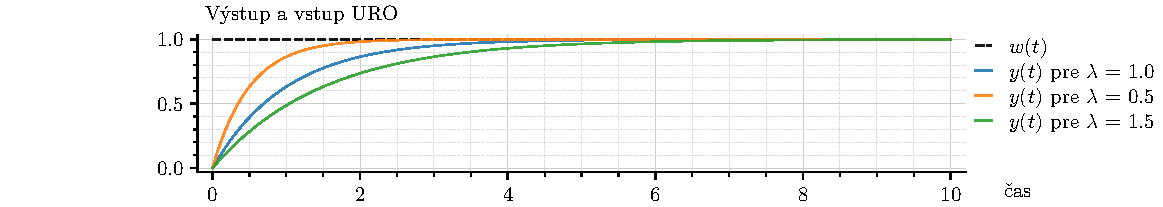
\includegraphics{MRS10_prikl_04_panel_wy.pdf}
    }

    \makebox[\textwidth][c]{%
    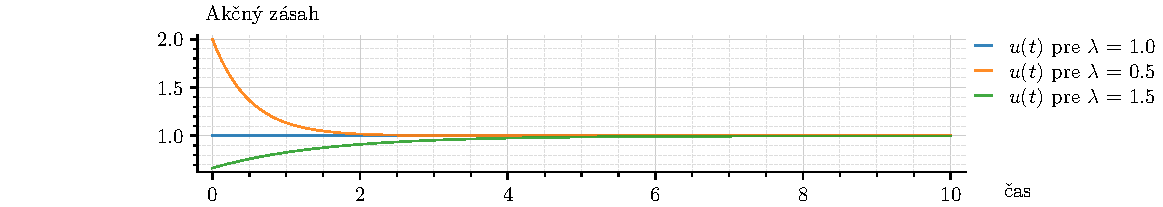
\includegraphics{MRS10_prikl_04_panel_u.pdf}
    }

    \figcaption{}
    \label{MRS08_prikl_04}
    }
    

\end{center}








\paragraph{Simulačný experiment 2}

Uvažujme prenosovú funkciu s parametrami $K=0,84$ a $T=6,66$.
\begin{align}
    G_S(s) = \frac{0,84}{6,66s+1}
\end{align}
Podľa \eqref{r0r1analyt} a pre $\lambda = 0,2$ majú parametre PI regulátora hodnoty:
\begin{equation} \label{r0r1analyt2}
    r_0 = 5,95 \qquad \text{a} \qquad r_{-1} = 0,89
\end{equation}
Výsledky simulácie regulácie na žiadanú hodnotu ($w(t) = 0,5$) sú na nasledujúcom obrázku (obr.~\ref{MRS08_prikl_05}).

\begin{center}

    \vbox{%
    \makebox[\textwidth][c]{%
    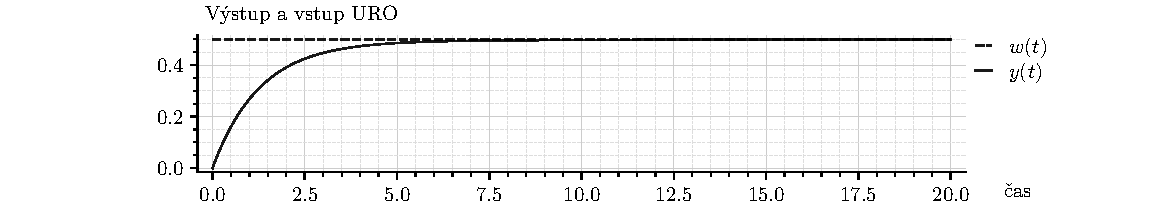
\includegraphics{MRS10_prikl_05_panel_wy.pdf}
    }

    \makebox[\textwidth][c]{%
    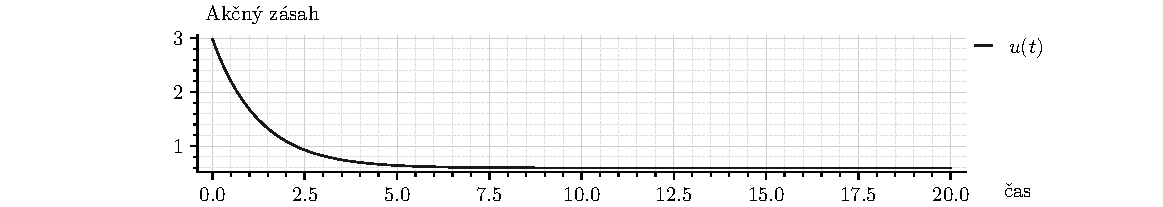
\includegraphics{MRS10_prikl_05_panel_u.pdf}
    }

    \figcaption{}
    \label{MRS08_prikl_05}
    }


\end{center}















\subsection{Metóda rozmiestňovania pólov}
\label{Metóda rozmiestňovania pólov}

Vzhľadom na to, že sa tu zaoberáme PID regulátorom je zrejmé, že póly, ktoré má zmysel rozmiestňovať, sú póly URO. Predpísaním pólov URO je možné stanoviť želanú výslednú dynamiku URO.


\subsection{Konkrétny príklad s PI regulátorom}

Pre ilustráciu uveďme príklad. Uvažuje sa model riadeného systému v tvare
\begin{align}
    G_S(s) = \frac{K}{T} \frac{1}{ \left(s+\cfrac{1}{T}\right)}
\end{align}
a PI regulátor s parametrami $P$ a $T_i$ 
\begin{align}
    G_R(s) = P \left( 1 + \cfrac{1}{T_i s}\right) = P \frac{ \left(s+\cfrac{1}{T_i}\right) }{s}
\end{align}
Výsledná prenosová funkcia URO bude druhého rádu. 

Nech želaným charakteristickým polynómom prenosovej funkcie URO je
\begin{align}
    Z(s) = s^2 + 2 b \omega_0 s + \omega_0^2
\end{align}
kde koeficient tlmenia $b$ a frekvencia $\omega_0$ sú voliteľnými parametrami. Ich voľbou sú jednoznačne určené korene polynómu $Z(s)$ a naopak. Ak by bol polynóm $Z(s)$ charakteristickým polynómom URO, potom by, samozrejme, išlo o rozmiestňovanie pólov URO voľbou parametrov $b$ a~$\omega_0$.







\paragraph{Stanovenie prenosovej funkcie URO}

Uvážme, že prenosová funkcia URO je
\begin{align} 
    G_{URO}(s) = \frac{G_{ORO}(s)}{1+G_{ORO}(s)} 
\end{align}
pričom v tomto prípade
\begin{equation}
    \begin{aligned}
        G_{ORO}(s) &= \frac{K}{T} \frac{1}{ \left(s+\cfrac{1}{T}\right)}  P \frac{ \left(s+\cfrac{1}{T_i}\right) }{s} \\
        &= \frac{KP}{T} \frac{\left(s+\cfrac{1}{T_i}\right)}{ \left(s+\cfrac{1}{T}\right) s}
    \end{aligned}
\end{equation}
Následne
\begin{equation}
    \begin{aligned}
        G_{URO}(s) 
        &= 
        \frac{%
            KP \left( s + \cfrac{1}{T_i}\right)
            }{%
            T \left( s + \cfrac{1}{T}\right) s + KP \left( s + \cfrac{1}{T_i}\right)
            }
        \\
        &=
        \frac{%
            KP \left( s + \cfrac{1}{T_i}\right)
            }{%
            T s^2 + s + KPs + \cfrac{KP}{T_i}
            }
        \\
        &=
        \frac{KP}{T}
        \frac{%
            \left( s + \cfrac{1}{T_i}\right)
            }{%
            s^2 + \left(\cfrac{1 + KP}{T}\right) s + \cfrac{KP}{TT_i}
            }
    \end{aligned}
\end{equation}
Prenosová funkcia $G_{URO}(s)$ je teda stanovená.





\paragraph{Povšimnutia}

Povšimnime si, že v ustálenom stave (teda $s \to 0$) platí
\begin{equation}
    \frac{y(\infty)}{w(\infty)} = \frac{\cfrac{KP}{TT_i}}{\cfrac{KP}{TT_i}} = 1
\end{equation}
Zosilnenie URO je teda jednotkové, čo je takpovediac samozrejmá požiadavka kladená na URO (môžu byť prípady kde sa to nevyžaduje).

Taktiež si povšimnime, že prenosová funkcia $G_{URO}(s)$ má vo všeobecnosti nulu, polynóm v čitateli je prvého stupňa. Poloha tejto nuly je daná parametrom regulátora $T_i$. Táto nula sa nevyhnutne prejaví pri regulačnom priebehu (napr. pri skokovej zmene želanej hodnoty). Inými slovami, táto nula nevyhnutne bude ovplyvňovať celkovú dynamiku URO. To môže byť nežiadúce, pretože želaná výsledná dynamika tu má byť daná len pólmi $G_{URO}(s)$. Ako zmierniť vplyv uvedenej nuly je nad rámec tohto učebného textu. Vyžaduje si to štrukturálnu zmenu samotného PID regulátora (metódy známe ako váhovanie žiadanej hodnoty) a tým by sa do istej miery pozmenila aj vyššie uvedená analýza vedúca na stanovenie prenosovej funkcie $G_{URO}(s)$.






\paragraph{Charakteristický polynóm URO}

Charakteristický polynóm URO je v tvare
\begin{equation}
    A_{URO}(s) = s^2 + \left(\cfrac{1 + KP}{T}\right) s + \cfrac{KP}{TT_i}
\end{equation}
Cieľom je aby sa tento polynóm zhodoval s $Z(s)$. Pre tento cieľ je možné vhodne stanoviť parametre regulátora $P$ a $T_i$.

\paragraph{Výpočet parametrov regulátora}

Pre zhodu $A_{URO}(s)$ a  $Z(s)$ musí platiť
\begin{align}
    \frac{1+KP}{T} &= 2b\omega_0 \\
    1 + KP &= 2b\omega_0 T \\
    KP &= 2b\omega_0 T - 1 \\
    P &=  \frac{2b\omega_0 T - 1}{K} \label{Pcomp}
\end{align}
a zároveň
\begin{align}
    \frac{KP}{TT_i} = \omega_0^2 
\end{align}
preto
\begin{align}
    \frac{2b\omega_0 T - 1}{TT_i} &= \omega_0^2  \\
    \omega_0^2 TT_i &= 2b\omega_0 T - 1 \\
    T_i &= \frac{2b\omega_0 T - 1}{\omega_0^2 T} \label{Ticomp}
\end{align}

Všimnime si, že ak majú byť parametre regulátora kladné, voliteľný parameter $\omega_0$ musí spĺňať $\omega_0 > \frac{1}{2bT}$.





\subsubsection{Simulačný experiment pre ilustráciu}

Pre uvedený príklad uvažujme konkrétne
\begin{align}
    G_S(s) = \frac{1}{s+1}
\end{align}
kde teda $K=1$ a $T=1$ sú parametre riadeného systému. 

Želané rozmiestnenie pólov stanovme voľbou parametrov
\begin{equation} 
    b = \frac{\sqrt{2}}{2}      \qquad \text{a} \qquad     \omega_0 = 2 \frac{1}{2bT}
\end{equation}
Podľa \eqref{Pcomp} a  \eqref{Ticomp} majú parametre PI regulátora hodnoty
\begin{equation} 
    P = 1      \qquad \text{a} \qquad     T_i = 0,5
\end{equation}
Póly URO (teda korene charakteristického polynómu URO) sú
\begin{equation} 
    s_{k1} = -1+j      \qquad \text{a} \qquad     s_{k2} = -1-j
\end{equation}
a nula URO (koreň polynómu v čitateli $G_{URO}(s)$) je
\begin{equation} 
    s_{n1} = -2   
\end{equation}
Simulácia regulácie na želanú hodnotu uvedená na obrázku~\ref{MRS08_prikl_06}.

\begin{center}

    \vbox{%
    \makebox[\textwidth][c]{%
    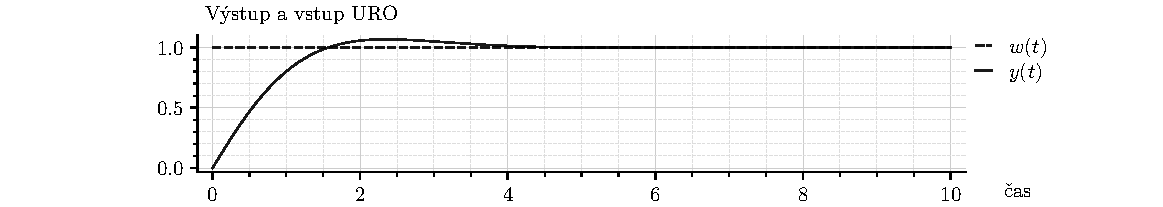
\includegraphics{MRS10_prikl_06_panel_wy.pdf}
    }

    \makebox[\textwidth][c]{%
    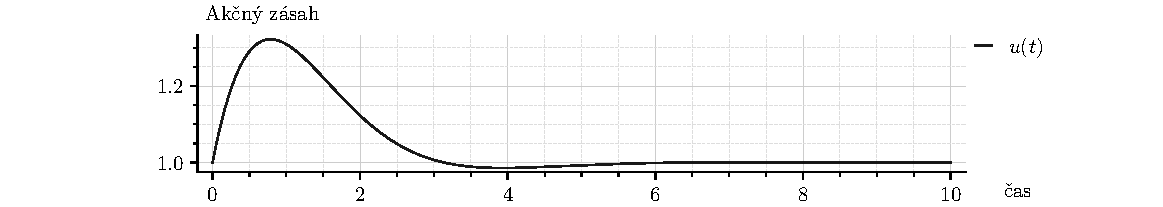
\includegraphics{MRS10_prikl_06_panel_u.pdf}
    }

    \figcaption{}
    \label{MRS08_prikl_06}
    }

\end{center}














\subsection{Metóda optimálneho modulu}
\label{Metóda optimálneho modulu}

Táto metóda vychádza z predstavy ideálnej prenosovej funkcie URO. Ideálne by bolo, ak by $G_{URO}(s) = 1$. To by totiž znamenalo, že signál predstavujúci želanú hodnotu $W(s)$ (alebo referenčný signál) by sa okamžite (bez akejkoľvek zotrvačnosti) preniesol na výstup URO $Y(s)$, keďže $Y(s) = G_{URO} W(s)$. Formálnejšie
\begin{equation}
    G_{URO}(s) = \frac{Y(s)}{W(s)}  \overset{!}{=} 1   \quad   \Longrightarrow  \quad y(t)=w(t) \ \forall t
\end{equation}
Toto je, samozrejme, nerealizovateľné. Nie je možné mať URO s nekonečne rýchlou dynamikou.


\paragraph{Modul $G_{URO}(j\omega)$}

Keďže $G_{URO}(s) = 1$ je nereálna požiadavka, Metóda optimálneho modulu je postavená na požiadavke týkajúcej sa modulu prenosovej funkcie $G_{URO}(s)$ namiesto požiadavky na prenosovú funkciu samotnú. Hovoríme o module v zmysle rovnakom ako keď hovoríme o komplexnom čísle. Výraz $G_{URO}(s)$ totiž je komplexné číslo. Vzhľadom na súvislosti vyplývajúce z Laplaceovej transformácie (a Fourierovej transformácie), o ktorých tu nebudeme hovoriť, má význam uvažovať $s = j\omega$, kde $j$ je komplexná jednotka a $\omega$ [rad/s] je frekvencia. Ak $s = j\omega$ tak $G_{URO}(j\omega)$ je takzvaná frekvenčná prenosová funkcia (podrobnosti sú nad rámec tohto učebného textu). 

V každom prípade, $G_{URO}(j\omega)$ je komplexné číslo. Modul tohto komplexného čísla sa označuje ako $ \left| G_{URO}(j\omega) \right| $.





\subsubsection{Princíp metódy}

Pre priblíženie hlavnej myšlienky metódy je možné konštatovať, že ak nemôžeme mať $G_{URO}(s) = 1$, tak nech aspoň modul tejto prenosovej funkcie nech je jednotkový.

Konkrétnejšie, pri Metóde optimálneho modulu je požiadavkou aby kvadrát modulu $G_{URO}(j\omega)$ bol jednotkový pre čo najväčší rozsah frekvencií $\omega$. Formálnejšie, kde modul označme $M$
\begin{equation}
    \left| G_{URO}(j\omega) \right|^2 = M^2(\omega) \overset{!}{=} 1
\end{equation}

Metóda ponúka nasledujúce riešenie uvedenej požiadavky. Platí
\begin{align}
    G_{URO}(j\omega) = \frac{G_{ORO}(j\omega)}{1+G_{ORO}(j\omega)} 
\end{align}
Ďalej platí
\begin{align}
    G_{ORO}(j\omega) = U(\omega) + jV(\omega)
\end{align}
kde $U(\omega)$ a $V(\omega)$ sú reálna a imaginárna časť komplexného čísla $G_{ORO}(j\omega)$. Samotné hodnoty $U$ a $V$ sú závislé od frekvencie $\omega$. Následne môžeme písať
\begin{equation}
    \begin{aligned}
        M^2(\omega) 
        &= \left| G_{URO}(j\omega) \right|^2 \\
        &= \left| \frac{G_{ORO}(j\omega)}{1 + G_{ORO}(j\omega)} \right|^2 \\
        &= \left| \frac{U(\omega) + jV(\omega)}{1 + U(\omega) + jV(\omega)} \right|^2 \\
        &=  \frac{ \left|U(\omega) + jV(\omega) \right|^2}{ \left|1 + U(\omega) + jV(\omega) \right|^2} \\
        &= \frac{ U^2(\omega) + V^2(\omega) }{1 + 2U(\omega) + U^2(\omega) + V^2(\omega)} 
    \end{aligned}
\end{equation}
Je zrejmé, že ak by platilo
\begin{equation}
    1+2U(\omega) = 0
\end{equation}
tak by tiež platilo
\begin{equation}
    M^2(\omega) = 1
\end{equation}

V tomto momente teda požiadavkou je aby
\begin{equation}
    U(\omega) = -\frac{1}{2}
\end{equation}
Inými slovami, reálna časť komplexného čísla $G_{ORO}(j\omega)$ má mať hodnotu $-\frac{1}{2}$.
\begin{equation}
    \Re \Bigl\{ G_{ORO}(j\omega) \Bigl\} = -\frac{1}{2} 
\end{equation}






\subsubsection{Postup}

Vzhľadom na uvedené je možné stanoviť nasledujúci postup.
\begin{itemize}[leftmargin=0pt, labelsep=3mm, itemsep=0pt]
    \item Je známa prenosová funkcia riadeného systému $G_S(s)$.
    \item Zvolí sa regulátor (štruktúra PID regulátora) a tým prenosová funkcia regulátora $G_R(s)$.
    \item Prenosová funkcia otvoreného regulačného obvodu je $G_{ORO}(s) = G_R(s) G_S(s)$.
    \item Za $s$ sa dosadí $j\omega$ a získa sa frekvenčná prenosová funkcia $G_{ORO}(j\omega)$.
    \item Stanový sa $\Re \bigl\{ G_{ORO}(j\omega) \bigl\}$, označme $U(\omega)$, pričom ide formálne o polynóm vzhľadom na premennú $\omega$. Vo výraze $U(\omega)$ sa vo všeobecnosti nachádzajú parametre riadeného systému (tie sú známe) a neznáme parametre regulátora (vo všeobecnosti to sú $r_0$, $r_{-1}$ a $r_1$).
    \item Parametre regulátora hľadáme riešením rovnice
    \begin{equation} \label{eq:aaa}
        U(\omega) = -\frac{1}{2}
    \end{equation}
    Ide o diofantickú rovnicu ($U(\omega)$ je polynóm vzhľadom na $\omega$). Riešenie hľadáme porovnaním koeficientov pri rovnakých mocninách $\omega$ na oboch stranách rovnice \eqref{eq:aaa}.
\end{itemize}





\subsubsection{Príklad}

Riadený systém
\begin{align}
    G_S(s) = \frac{K}{Ts+1}
\end{align}
Regulátor
\begin{align}
    G_R(s) = \frac{r_0 s + r_{-1}}{s}
\end{align}
Otvorený regulačný obvod
\begin{align}
    G_{ORO}(s) = \frac{K r_0 s + K r_{-1}}{T s^2 + s}
\end{align}
\begin{equation}
    \begin{aligned}
        G_{ORO} (j\omega)
        &=
        \frac{K r_0 j\omega + K r_{-1}}{T (j\omega)^2 + j\omega} 
        \\
        &=
        \frac{K r_0 j\omega + K r_{-1}}{ -T \omega^2 + j\omega} \cdot \frac{-T\omega^2 - j\omega}{-T\omega^2 - j\omega}
        \\
        &=
        \frac{K r_0 j \omega (-T\omega^2 - j^2 K r_0 \omega - K r_{-1} T \omega^2 - j K r_{-1} \omega   }{ \left( -T\omega^2 \right)^2 + \omega^2   }
        \\
        &=
        \frac{K r_0 \omega - K r_{-1} T \omega^2 + j \left( K r_0\omega (-T\omega^2) - K r_{-1} \omega   \right)   }{ T^2\omega^4 + \omega^2   }
    \end{aligned}
\end{equation}
Preto
\begin{align}
    \Re \bigl\{ G_{ORO}(j\omega) \bigl\} = \frac{K r_0 \omega - K r_{-1} T \omega^2    }{ T^2\omega^4 + \omega^2   }
\end{align}
Neznáme parametre $r_0$ a $r_{-1}$ hľadáme riešením rovnice
\begin{align}
    \frac{K r_0 \omega - K r_{-1} T \omega^2    }{ T^2\omega^4 + \omega^2   } &= -\frac{1}{2} \\
    K r_0 \omega - K r_{-1} T \omega^2     &= -\frac{1}{2} \left( T^2\omega^4 + \omega^2  \right) \\
    K r_0 \omega - K r_{-1} T \omega^2     &= -\frac{1}{2} T^2\omega^4 -\frac{1}{2} \omega^2  
\end{align}
Ak uvážime koeficienty pri $\omega$ a $\omega^2$ potom
\begin{align}
    K r_0 &= 0 \\
    - K r_{-1} T &= -\frac{1}{2}
\end{align}
a teda
\begin{align}
    r_0 &= 0 \\
    r_{-1}  &= \frac{1}{2KT}
\end{align}
Tým sme určili parametre prenosovej funkcie regulátora, pričom pre tento prípad ide o I regulátor (P zložka má nulový parameter).









\paragraph{Simulačný experiment}


Uvažujme prenosovú funkciu s parametrami $K=0,84$ a $T=6,66$.
\begin{align}
    G_S(s) = \frac{0,84}{6,66s+1}
\end{align}
Podľa výsledku vyššie majú parametre PI regulátora hodnoty:
\begin{equation} \label{r0r1analyt3}
    r_0 = 0 \qquad \text{a} \qquad r_{-1} = 0,089
\end{equation}
Výsledky simulácie regulácie na žiadanú hodnotu ($w(t) = 0,5$) sú na nasledujúcom obrázku (obr.~\ref{MRS08_prikl_07}).

\begin{center}

    \vbox{%
    \makebox[\textwidth][c]{%
    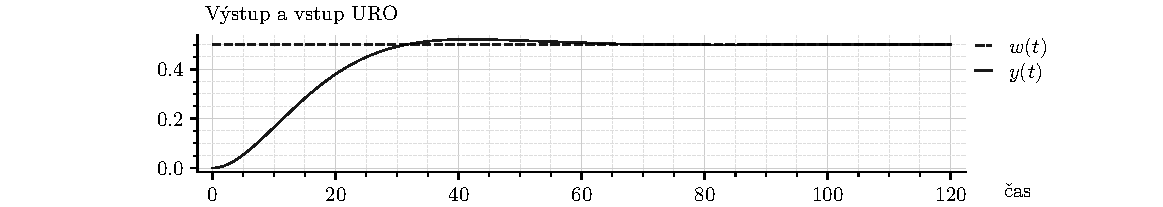
\includegraphics{MRS10_prikl_07_panel_wy.pdf}
    }

    \makebox[\textwidth][c]{%
    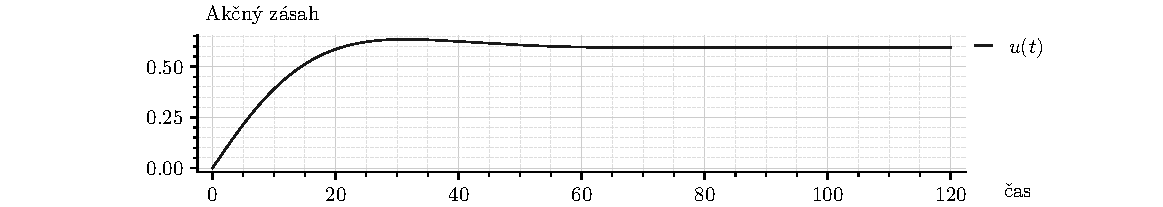
\includegraphics{MRS10_prikl_07_panel_u.pdf}
    }

    \figcaption{}
    \label{MRS08_prikl_07}
    }

\end{center}







\subsubsection{Poznámky k metóde}


\begin{itemize}[leftmargin=0pt, labelsep=3mm, itemsep=0pt]
    \item Metóda nezaručuje stabilitu URO. Tú je potrebné vyšetriť následne po získaní parametrov prenosovej funkcie regulátora.
    \item Metóda nezaručuje existenciu riešenia rovnice $U(\omega) = -\frac{1}{2}$ (neznáme parametre  $r_0$, $r_{-1}$ a $r_1$) pre akúkoľvek kombináciu štruktúry PID a prenosovej funkcie riadeného systému.
    \item Výsledok metódy je možné interpretovať ako tvarovanie frekvenčnej charakteristiky otvoreného regulačného obvodu (ORO) tak, aby pre čo najväčší rozsah frekvencií $\omega$ platilo, že frekvenčná charakteristika ORO je zhodná s takou priamkou v komplexnej rovine, ktorá je rovnobežná s imaginárnou osou a prechádza bodom $-0,5 + j0$.
    \item Metódu je možné čiastočne zovšeobecniť ak sa prenosová funkcia riadeného systému upraví do tvaru
    \begin{equation}
        G_S(s) = \frac{K}{1 + a_1s + a_2s^2 + a_3s^3 + \ldots}
    \end{equation}
    Potom, pre I regulátor platí
    \begin{equation}
        r_{-1} = \frac{1}{2K} \frac{1}{a_1}
    \end{equation}
    pre PI regulátor platí
    \begin{equation}
        \begin{bmatrix}
            a_1 & -1 \\ a_3 & -a_2
        \end{bmatrix}
        \begin{bmatrix}
            r_{-1} \\ r_0
        \end{bmatrix}
        =
        \frac{1}{2K}
        \begin{bmatrix}
            1 \\ -a_1^2 + 2 a_2
        \end{bmatrix}
    \end{equation}
    pre PD regulátor platí
    \begin{equation}
        \begin{bmatrix}
            -a_2 & a_1 \\ -a_4 & a_3
        \end{bmatrix}
        \begin{bmatrix}
            r_{0} \\ r_1
        \end{bmatrix}
        =
        \frac{1}{2K}
        \begin{bmatrix}
            -a_1^2 + 2 a_2 \\ a_2^2 - 2 a_1a_3 + 2a_4
        \end{bmatrix}
    \end{equation}
    a pre PID regulátor platí
    \begin{equation}
        \begin{bmatrix}
            a_1 & -1 & 0 \\ a_3 & -a_2 & a_1 \\ a_5 & -a_4 & a_3
        \end{bmatrix}
        \begin{bmatrix}
            r_{-1} \\ r_0 \\ r_1
        \end{bmatrix}
        =
        \frac{1}{2K}
        \begin{bmatrix}
            1 \\ -a_1^2 + 2 a_2 \\ a_2^2 - 2 a_1a_3 + 2a_4
        \end{bmatrix}
    \end{equation}
\end{itemize}












\section{O ukazovateľoch kvality PCH URO}

Typicky sa pri posudzovaní kvality uzavretého regulačného obvodu (URO) využíva prechodová charakteristika (PCH). Vstupom URO je želaná hodnota (referenčný signál) $w(t)$ a výstupom je výstupná veličina riadeného systému $y(t)$. Prechodová charakteristika URO je teda priebeh výstupnej veličiny po skokovej zmene želanej hodnoty.

V tomto prípade teda ide takpovediac o kvalitu URO pri prechodných dejoch.

Prechodová charakteristika URO v mnohých prípadoch vykazuje tlmené oscilácie pred dosiahnutím ustáleného stavu. Príkladom nech je obr.~\ref{MRS10_kvalitaPCHURO_panel_wy}.

\begin{center}

    \vbox{%
    \makebox[\textwidth][c]{%
    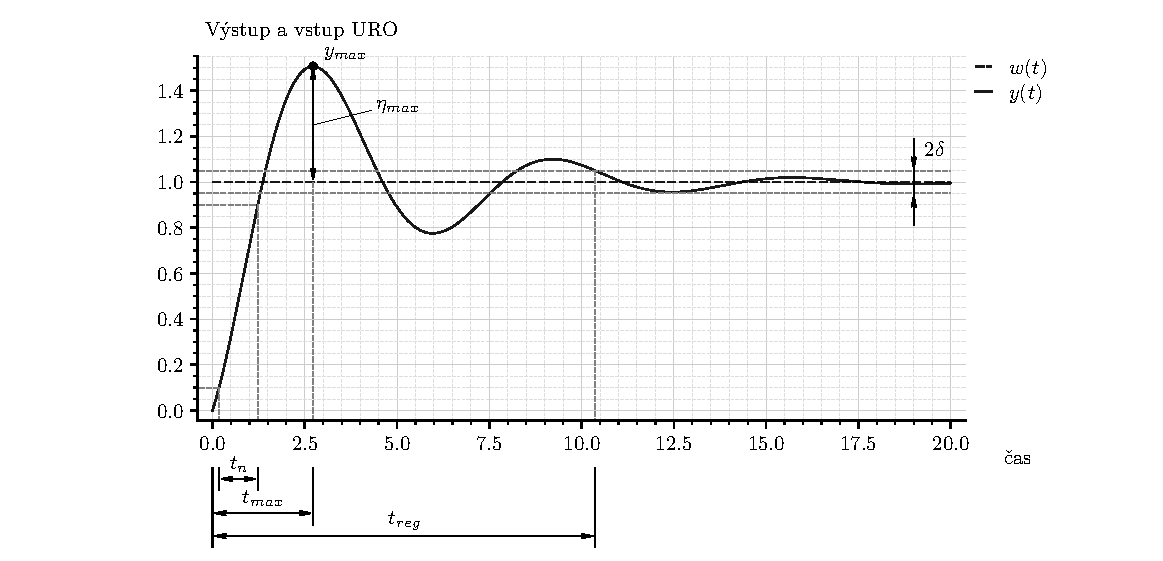
\includegraphics{MRS10_kvalitaPCHURO_panel_wy.pdf}
    }


    \figcaption{}
    \label{MRS10_kvalitaPCHURO_panel_wy}
    }

\end{center}

\noindent
Z prechodovej charakteristiky URO je možné odčítať niekoľko hodnôt, ktoré sa používajú ako ukazovatele kvality URO (pri prechodnom deji):

\begin{itemize}[leftmargin=0pt, labelsep=3mm, itemsep=0pt]
    \item Maximálne preregulovanie $\eta_{max}$
    \item Doba regulácie $t_{reg}$ (alebo čas regulácie)
    \item Doba nábehu $t_n$ (alebo čas nábehu)	
\end{itemize}

\paragraph{Maximálne preregulovanie}

Maximalne preregulovanie $\eta_{max}$ sa typicky udáva v percentách pričom $100$ \% je ustálená hodnota výstupnej veličiny $y(\infty)$. Maximálne preregulovanie je
\begin{equation}
    \eta_{max} = \frac{y_{max} - y(\infty)}{y(\infty)} \times 100 \%
\end{equation}
kde $y_{max}$ je maximálna hodnota výstupnej veličiny $y(t)$, ktorá nastala v čase $t_{max}$ po skokovej zmene želanej hodnoty.

\paragraph{Doba regulácie}

Doba regulácie $t_{reg}$ je čas, ktorý uplynie od skokovej zmeny želanej hodnoty kým sa výstupná veličina dostane do pásma necitlivosti a ostane v ňom.

Pásmo necitlivosti je určené percentom z ustálenej hodnoty výstupnej veličiny $y(\infty)$. Toto percento je typicky $2$ až $5$ \%, prípadne aj viac v závislosti od konkrétnej aplikácie. Uvažuje sa teda pásmo so stredom v $y(\infty)$ a šírkou $2 \delta$ pričom $\delta$ je daná uvedeným percentom, napríklad
\begin{equation}
    \delta = 0,05  \cdot y(\infty) 
\end{equation}

\paragraph{Doba nábehu}

Ukazovateľom rýchlosti regulácie môže byť aj takzvaná doba nábehu $t_n$. Je to čas, za ktorý sa výstupná veličina $y(t)$ zvýši z $10$ \% na $90$ \% svojej ustálenej hodnoty $y(\infty)$. Používajú sa aj iné percentá, napríklad $5$ a $95$ \% alebo $0$ a $100$ \%, opäť v závislosti na aplikácii.










% \section{Otázky a úlohy}


% \begin{enumerate}[leftmargin=0pt, labelsep=3mm, itemsep=0pt]


%     \item Schematicky znázornite všeobecný regulačný obvod, opíšte bloky a~signály, z~ktorých pozostáva.

%     \item Vysvetlite pojem \emph{regulačná odchýlka}.

%     \item Schematicky znázornite lineárny uzavretý regulačný obvod, opíšte prenosové funkcie a~signály (L-obrazy signálov), z~ktorých pozostáva.

%     \item Vysvetlite pojem \emph{prenosová funkcia otvoreného regulačného obvodu}.

%     \item S využitím algebry prenosových funkcii odvoďte prenosovú funkciu regulačnej odchýlky v klasickom lineárnom URO.

%     \item Majme lineárny uzavretý regulačný obvod s uvažovaním poruchovej veličiny $D(s)$ ako je znázornené na obr.:

%     \noindent
%     \makebox[\textwidth][c]{%
%     % 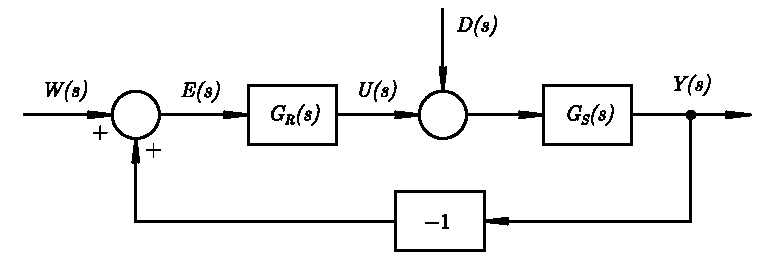
\includegraphics[scale=0.9]{schLinURO_basic_porucha.pdf}
%     \input{../fig_standalone/schLinURO_basic_porucha.pdf_tex}
%     }

%     \noindent
%     S využitím algebry prenosových funkcií odvoďte prenosovú funkciu definovanú pomerom L-obrazov $\frac{Y(s)}{D(s)}$ pri $W(s) = 0$.



%     \item Stručne opíšte PID regulátor.

%     \item Napíšte prenosovú funkciu PID regulátora.

%     \item Nakreslite blokovú schému PID regulátora.

%     \item Uvažujte klasický lineárny URO, kde $\displaystyle G_R(s) = r_0$ a $\displaystyle G_S(s) = \frac{K}{Ts + 1}$.
%     \begin{enumerate}
%         \item Nájdite prenosovú funkciu URO a vhodne komentujte postup.
%         \item Určte veľkosť trvalej regulačnej odchýlky ak $w(t) = 1$.
%     \end{enumerate}

%     \item Uvažujte klasický lineárny URO, kde $\displaystyle G_R(s) = r_0 + \frac{r_{-1}}{s}$ a $\displaystyle G_S(s) = \frac{K}{Ts + 1}$.
%     \begin{enumerate}
%         \item Nájdite prenosovú funkciu URO a vhodne komentujte postup.
%         \item Určte veľkosť trvalej regulačnej odchýlky ak $w(t) = 1$.
%     \end{enumerate}

%     \item Uvažujte klasický lineárny URO, kde $\displaystyle G_R(s) = r_0 + \frac{r_{-1}}{s}$ a $\displaystyle G_S(s) = \frac{1}{s}$.
%     \begin{enumerate}
%         \item Nájdite prenosovú funkciu URO a vhodne komentujte postup.
%         \item Určte veľkosť trvalej regulačnej odchýlky ak $w(t) = 1$.
%         \item Nájdite podmienku, ktorá musí byť splnená, aby prechodová charakteristika URO bola aperiodická.
%     \end{enumerate}






% \end{enumerate}



































\end{document}
